\documentclass{emulateapj} 
\usepackage{amsmath}
\usepackage{float}
\usepackage{natbib}

%\usepackage{csvsimple}

%\usepackage[toc\documentclass{emulateapj} 
\usepackage{amsmath}
\usepackage{float}
\usepackage{natbib}
\usepackage{hyperref}
%\usepackage{csvsimple}

\newcommand{\kms}{\ensuremath{{\rm km~s}^{-1}}}
\newcommand{\oxab}{\ensuremath{12~+~\log(O/H)}}
%\usepackage[toc\documentclass{emulateapj} 
\usepackage{amsmath}
\usepackage{float}
\usepackage{natbib}
\usepackage{hyperref}
%\usepackage{csvsimple}

\newcommand{\kms}{\ensuremath{{\rm km~s}^{-1}}}
\newcommand{\oxab}{\ensuremath{12~+~\log(O/H)}}
%\usepackage[toc\documentclass{emulateapj} 
\usepackage{amsmath}
\usepackage{float}
\usepackage{natbib}
\usepackage{hyperref}
%\usepackage{csvsimple}

\newcommand{\kms}{\ensuremath{{\rm km~s}^{-1}}}
\newcommand{\oxab}{\ensuremath{12~+~\log(O/H)}}
%\usepackage[toc\input{Metallicity_MCuncertainties.tex}
%,page]{appendix}
%\usepackage{amsmath}
%\usepackage{amssymb}
%\usepackage{verbatim}
%\usepackage{graphicx}
%\usepackage{epsfig}
%\usepackage{morefloats}
%\usepackage{float}
%\usepackage{lipsum}
%\usepackage{subfigure}
%\usepackage{longtable}
%\usepackage{lipsum} 
%\usepackage{rotating}
%\usepackage{wasysym}

\begin{document}
\title{Monte Carlo Method for Calculating Uncertainty in Oxygen Abundance from Strong-Line Flux Measurements}

\author{Author order to be determined: Maryam Modjaz\altaffilmark{1}, Federica B. Bianco\altaffilmark{1}, Seung Man Oh\altaffilmark{1,2}, David Fierroz\altaffilmark{1}, Yuqian Liu\altaffilmark{1}, Lisa Kewley\altaffilmark{3,4}}
\altaffiltext{1}{Center for Cosmology and Particle Physics, New York University, 4 Washington Place, New York, NY 10003, USA}
 \altaffiltext{2}{NYU Abu Dhabi PO Box 129188 Abu Dhabi, UAE}
 \altaffiltext{3}{Australian National University, Research School for Astronomy \& Astrophysics, Mount Stromlo Observatory, Cotter Road, Weston, ACT 2611, Australia }
 \altaffiltext{4}{ Institute of Astronomy, University of Hawaii, 2680 Woodlawn Drive, Honolulu, HI 96822, USA}
 
 
\begin{abstract}
\textbf{MODIFY \& FINALIZE AT THE END:} We present an open-source Python code for the determination of the strong-emission-line estimators of oxygen abundance in the standard scales, based on the original IDL-code in \citet{kewley02}. The standard strong line Metallicity scales and diagnostics \text{IMPROVE} have been used to estimate metal abundance through emission line ratios. Here we introduce a Monte Carlo resampling of these methods in order to better characterize an oxygen abundance confidence region.  We output median values, 16th and 84th percentile confidence regions, for various standard metallicity diagnostics, and, when possible, for reddening E(B-V). We produce Monte Carlo parameter distributions for the oxygen abundance and when possible for reddening E(B-V). We test our code on emission lines measurements from a sample of galaxies ($z<0.15$) and compare our metallicity results with those from previous methods. We show that our metallicity estimates are consistent with previous methods but yields smaller uncertainties. The code is open source and can be found at www.github.com/nyusngroup/ \textbf{
(add repo and DOI)}.
\end{abstract}
 
\section{Introduction}
The low quantity of carbon, oxygen, nitrogen, sulfur and iron among other elements provide a splash of color to the otherwise dominating greyscape of hydrogen and helium in the stars and gas of galaxies. Nevertheless, even the minute presence of heavy elements (all elements heavier than H and He, also called metals or collectively metallicity) is important for many areas of astrophysics. For example, \citet{johnson12} suggest that if it was not for the relatively high metallicity level in our Solar System, planet formation may not have been possible. With $Z$ representing the mass fraction of metals, for our own Sun the value is measured to be  Z=0.0153 \citep{chaffau11}, though there are others who suggest a lower solar metallicity of $Z=0.0134$ in particular because of oxygen \citep{asplund09_rev,grevesse10}\footnote{Note that these abundances refer to the current abundances in the sun, which are lower than the value with which the sun was formed 4.56 Gyr ago, since diffusion at the bottom of the convection zone has decreased metallicity over time \citep{grevesse10}.}. Furthermore, when properly observed and estimated, metallicity measurements of galaxies can tightly constrain models of galaxy formation and evolution (e.g., \citealt{kewley08} and references therein), tas well as shed light on the metallicity dependence and production conditions for different types of SNe and long-duration GRBs (e.g., \citealt{modjaz08_Z,levesque10_grbhosts,anderson10,modjaz11,kelly12,sanders12,lunnan14,leloudas14}), to just name a few examples.

%chaffau Z=0.0209 12+log=O/H) = 8.76�0.07 i
%Small variations in chemical abundance can often be critical indicators for stellar and galactic properties like age and activity.
%Metals are produced in the cores of stars during their fusion lifecycle but also during the extreme conditions of stellar explosions. For example, the majority of iron comes from thermonuclear explosions (SN Ia) while nearly all of oxygen is the result of core collapse (SN Ib, Ic, \& II). Since new stars are born from the clouds these explosions produce, metallicity will increase with each passing generation. Stars like our Sun, which are results of multiple generations of star formation, are often found in the more active parts of the galaxy, such as the disk, and are referred to as Population I stars. Population I stars have higher metallicity than older Population II stars, which are also present in the disk but are the exclusive members of the low activity galactic halo. Population III stars would be first generation stars with zero metallicity, but have yet to be observed.
%Besides age, metallicity also influences stellar temperature. Metals are more effective at absorbing energy coming from the interior of the star in the stellar atmosphere so their presence increases the stellar opacity. With greater absorption and opacity the radius expands to a size larger than it would be without metals and this larger size results in a cooler effective temperature. While metallicity can help indicate age or activity it's temperature and density dependencies require parameterization to properly be estimated.

However, for almost all astronomical objects, metallicity cannot be measured directly. The oxygen abundance in the gas-phase is the canonical choice of metallicity indicator for interstellar medium (ISM) studies, since oxygen is the most abundant metal and only weakly depleted onto dust grains (in contrast to refractory elements such as Mg, Si, Fe, with Fe being depleted by more than a factor of 10 in Orion; see \citealt{simondiaz11-orion}). The oxygen abundance\footnote{We note that in many cases in the literature, including here, the terms metallicity and oxygen abundance are used interchangeably.} is expressed as  $12 + \log_{10}(\frac{O}{H})$, where $O$ and $H$ represent the number of Oxygen and Hydrogen atoms, respectively. Importantly, oxygen exhibits very strong nebular lines in the optical wavelength range of HII regions (e.g., \citealt{pagel79,osterbrock89,tremonti04}), and thus, many different diagnostic techniques, relying on different lines, have been developed (e.g., \citealt{kewley02,pettini04,kobulnicky04,kewley08}), which are discussed in the next section.

\subsection{The different oxygen abundance diagnostics}
Here we present a brief overview of the various observational methods for measuring the gas-phase oxygen abundance - however, for a full discussion with all the caveats we encourage the reader to see reviews by e.g. \citet{stasinska02,kewley08,moustakas10,stasinska10,dopita13,blanc15}.
The so-called ``classical'' way to estimate the oxygen abundance is the electron temperature ($T_e$) method, which estimates the electron temperature and density of the nebula using a number of oxygen lines with different ionization states, including the auroral [OIII] $\lambda$4363 line, to then directly estimate the OII and OIII abundances to obtain the total oxygen abundance, after correcting for the unseen stages of ionization. However, the auroral [OIII] $\lambda$4363 line is very weak, even in low-metallicity environments, and saturates at higher metallicity (since at higher metallicities the cooling is dominated by the Oxygen NIR fine structure lines) $-$ thus, other methods had to be developed that use other, stronger lines, in the spectra of HII regions. These are called strong-line methods and are the subject of this manuscript. Strong-line methods can be categorized into two types: theoretical methods, that rely on calibrating various observed line ratios using photoionization methods (basically theoretically simulating HII regions, using stellar model atmospheres, stellar population synthesis and photoionization models) and empirical ones that calibrate various observed strong line ratios using observed $T_e$-based metallicities. While historically there have been large systematic offsets between the $T_e$ method and the strong line methods, \citet{dopita13} demonstrated that the $T_e$ method gives the same results as the strong line methods, if the energy distribution of the electrons in the HII regions is assumed to not be a simple Maxwell-Boltzmann distribution (as assumed in prior works), but a more realistic $\kappa$ distribution, as observed in solar system astrophysical plasma. They also find that the effect of the $\kappa$ distribution on the strong-line methods is minor.


For the theoretical strong-line method, one ratio that is commonly used to determine the metallicity of galaxies is ([OII] $\lambda 3727$ $+$ [OIII] $\lambda 4959,\lambda 5007$)$/$H$_\beta$ \citep{pagel79} and is referred to as R23. The drawback of this method is that it is double-valued with metallicity, and thus other line ratios need to be used to break the degeneracy between the high values ("upper branch") and the low values ("lower branch") of the R23 metallicities. Furthermore, \citet{kewley02} showed the importance of ionization parameter, which can be physically understood to correspond to the maximum velocity of an ionized front that can be driven by the local radiation field of hot massive stars that are ionizing the ISM gas. This ionization parameter needs to be taken into account in the various strong-line methods, as HII regions at the same metallicity but with different ionization parameters produce different line strengths. Calibrations of R23 by \citet{mcgaugh91} (hereafter M91) and by \citet{kewley02} (hereafter KD02) use different theoretical photoionization models and take the ionization parameter into account, while other calibrations such as of \citet{zaritsky94} (hereafter Z94) do not. Thus, Z94 is mostly valid for only metal-rich galaxies.  M91 and KD02 use an iterative process to break the R23 degeneracy  (KD02 uses different ratios [NII]$/$[OII] and [NII]$/$H$_\alpha$) and to also constrain the ionization parameter $q$ in order to arrive at the metallicity estimate.

%The most direct way to estimate metallicity in spectra is to measure line fluxes absorbed or emitted by metals and non-metals. While iron lines may be present in stellar spectra, iron is less commonly found in gaseous nebulae than oxygen is. Not only is oxygen more abundant but it emits several strong lines ([OI] $\lambda 6300$, [OII] $\lambda 3727,7318,7324$, [OIII] $\lambda 4363, 4959, 5007$) visible at optical wavelengths that can also be used to quantify temperature and density. For this reason 
%While the ratio of oxygen to hydrogen line flux correlate with metallicity, the ratio of two [OIII] lines, one auroral $\lambda 4363$ and the other an excitation line at $\lambda 5007$ can be used to determine what is called the Ionization Correction Factor (ICF) (Kewley \& Dopita 2002).
As to empirical strong-line methods, the most commonly used one is that by \citet{pettini04} (hereafter PP04). PP04 used HII regions with $T_e$-based metallicities to derive empirical fits to strong-line ratios, and introduce the line ratios of ([NII]$/$H$_\alpha$ (N2) and ([OIII]$/$H$_\beta$)$/$([NII]$/$H$_\alpha$ (O2N2) as metallicity diagnostics. Since PP04-N2 employs two closely spaced lines (Halpha and NII), which are not affected by stellar absorption, nor uncertain reddening, and are easily observed in one simple spectroscopic setup, it has become an often-used scale for at least low-z SN host galaxy studies (e.g. see metal-analysis by e.g,. \citealt{sanders12,modjaz12_proc,leloudas14}). However, it is important to remember that this scale has a number of short-comings: it does not take into account the impact of the ionization parameter, it was initially derived based on only 137 extragalactic HII regions, and the nitrogen emission line employed saturates at high metallicity (\textbf{CHECK!}), and thus this method may not be well-suited for high-metallicity galaxies. An updated calibration by \citet{marino13} based on many more Te-based metallicities (almost three time larger that that of PP04) derives a significantly shallower slope between O3N2 index and oxygen abundance than the PP04 calibration.


As it can be seen, each scale has different advantages and disadvantages and should be used in different metallicity regimes (see detailed discussion in e.g.,  \citealt{kewley02,stasinska02,kewley08,moustakas10,dopita13,blanc15}). Thus, this open-source code outputs the oxygen abundance in the main 6 metallicity scales (for which the KD02 diagnostic has four outputs and the PP04 diagnostic has two outputs). While there is a long-standing debate about which diagnostic to use, as there are systematic metallicity offsets between different methods (recombination lines vs.  strong-line method vs. ``direct'' $T_e$ method, see the above sources), \emph{\bf the relative metallicity trends can be considered robust, if the analysis is performed self-consistently in the same scale, and trends are seen across different scales \citep{kewley08,moustakas10}}. Note however, that while there are conversion values between different scales \citep{kewley08}, they apply for large data sets, since those conversion values were derived based on ten thousands of SDSS galaxies, and thus should be used with caution (or not at all) for smaller samples. In addition, one should note that there is a debate about the value of the solar oxygen abundance \citep{asplund09_rev,chaffau11}, such that the absolute oxygen calibration is still uncertain.




Here we introduce the open-source python code "". pro .. In \S~\ref{method_sec} we describe our method, the input and output values of the code. In \S~\ref{comp_sec}, we compare our method of obtaining abundance uncertainties to previous methods in the literature. 
%\begin{figure}[H]
%\epsscale{1.0} 
%\begin{center}
%\includegraphics[width=0.89\columnwidth]{fig1.png} 
%\caption{Example of a sampled Gaussian. 50,000 points from a Gaussian distribution were selected in this case}
%\label{f1}
%\end{center}
%\end{figure}


\section{Description of Metallicity code}\label{method_sec}


\begin{figure*}[!HT]
%\epsscale{0.6}
\begin{center}
\centerline{
\includegraphics[width=0.95\columnwidth]{exampledata_n2000_KD02comb_1.pdf}
%exampledata_n50000_KD02comb_updated_1.ps}
\includegraphics[width=0.95\columnwidth]{exampledata_n2000_PP04_O3N2_1.pdf}}
%exampledata_n50000_PP04_O3N2_1.ps}
\vspace{0.2in}
\centerline{
\includegraphics[width=0.95\columnwidth]{exampledata_n2000_M91_1.pdf}
% exampledata_n50000_M91_1.ps}
\includegraphics[width=0.95\columnwidth]{exampledata_n20000_E(B-V)_1.pdf}}
%exampledata_n50000_EBV_1.ps}

\caption{WILL UPDATE WITH NEW FIGURES BASED ON A PUBLISHED SN WITH SIGNFICANT E(B-V) AND WRITE MORE TEXT. Metallicity and reddening ($E(B-V)$) parameter distributions based on example data (namely, emission line data of the HII regions at the position of SN~2008D, published in \citet{modjaz11}, based on $N$=20,0000 samples. The median value is shown with the dashed lines, while the 16th till 84th confidence region is shaded in tan color. The shown metallicity scales are  by \citet{kewley02}, updated by \citet{kewley08} (KD02combupdated), \citet{pettini04}, using OIII and NII  (PP04-O3N2) and \citet{mcgaugh91} (M91). These are the same plots that are outputted by the code, which produces such plots for all scales (namely those of s\textbf{LIST THEM ALL}). The legend also includes the ID number of }
 \label{metallicity_distribution}
\end{center}
\vspace{-0.5in}
\end{figure*}


For computing oxygen abundances, we use the iterative code by \citet{kewley02}, which has been updated in \citet{kewley08} and reflects .. \textbf{LISA: YOUR INPUT HERE:what is the update??} which was initially written in IDL.  We translated the code into python, added the new feature of obtaining uncertainties on the metallicity outputs via Monte Carlo resampling, and made it open source via github, as we explain below.

We assume that the observed emission lines to be used to indicate metallicity originate in HII regions and are not due to non-thermal excitation by e.g., AGN or interstellar shocks from SNe or stellar winds.  Tests to exclude data contaminated by such non-thermal sources should be executed using the recommended line ratios by e.g., \citealt{baldwin81,kauffmann03,kewley06_sdss} prior to running this code. Furthermore these lines should have all the correct calibration (at least correct relative calibration) and should have a signal-to-noise ratio (S/N) of at least 3. The latter is important for the success of the Monte Carlo resampling technique as described below.

\subsection{Input and Output of code}
Emission line flux values are fed into our Python implementation as in the original IDL code by \citet{kewley02}, hereafter referred to as IDLKD02. The inputs are emission line flux values and their uncertainties for the following lines: H$\alpha$, H$\beta$, [OI] 6300, [OII] 3727, [OIII] 4959, [OIII] 5007, [NII] 6584, [SII] 6717, [SII] 6731, SIII 9532, and SIII 9096 \textbf{CHECK AT THE END WITH CODE!} and their uncertainties (consult the README.md in the github repository for details about the input format). If the fluxes for the specified lines are not available, the entry is left to 0 \textbf{FED: we should do NaN!???} and the outputted oxygen abundance scales will be in only metallicity scales that use the provided line fluxes. As part of the code, the inputted line fluxes are corrected for reddening by using the observed Balmer decrement, for which H$\alpha$ and  H$\beta$ flux values need to be provided. We assume case B recombination, and thus the standard value of 2.86 as the
intrinsic H$\alpha$/H$\beta$ ratio \citep{osterbrock89}, and apply the standard Galactic reddening law with $R_V$ = 3.1 \citep{cardelli89}. However, the user can choose other extinction laws and $R_V$ values, if desired, given the code's open-source nature.

While other parameters, such as the ionization parameter $q$ and the electron density (using the SiII lines) are computed as long as the necessary lines are provided, they are not outputted in the current version of our code $-$ however, the reader is welcome to easily modify the code to suite their needs, given it's an open-source code.

As output, we obtain metallicity values and their uncertainties in the following calibrations, as discussed in detail in \citet{kewley02,kewley08}: \citet{kewley02}(KD02, for the 4 following computations: R23, using the NIIOII ratio, using the NII/Halpha ratio, and a combined method that uses the optimal method given the input line fluxes), \citet{mcgaugh91} (M91), \citet{zaritsky94} (Z94), \citet{pilyugin01} (P01), \citet{denicolo02} (D02), 
\citet{pettini04} (2 computations: PP04-N2, PP04-O3N2) \textbf{CHECK WITH FINAL CODE - ALSO CHECK whether P01 is P01 or P05 by looking at the code}. If the line fluxes necessary for specific scales are not provided, the output  metallicities will default to -1, if the errors in he measurements are not provided, the code will specify that it cannot create a measurement distribution and determine a confidence interval.



\subsection{Computing Uncertainties}
The novel aspect of our work is that for every set of input line measurements we introduce a Monte Carlo (MC) resampling method to obtain iterations via random sampling within the measurement errors, and thus we obtain a robust result for error estimation (e.g., \citealt{efron79,hastie09,andrae10}). 

Given a data set with error bars from which certain parameters are estimated, Monte Carlo resampling generates synthetic data samples drawing from a given distribution. 
Here we draw synthetic data from a Gaussian distribution centered on each measured line flux value, with standard deviation corresponding to the measurement error. The implicit assumption is made, of course, that the line flux error is Gaussian distributed in nature\footnote{The user may wish to provides their own probability distribution for the emission line uncertainties, and easily modify the code to suite their needs.}. 

% FED: because we vectorize, we actually do not do this sample by sample so we cannot say ``Every iteration''
For each metallicity scale, for each of $N$  values chosen randomely within the relevant emission line distributions we run the calculations that derives the metallicity.
This effectively simulates conducting multiple experiments when repeating observations is impractical or impossible, as in the case of the emission line flux data, and thus generates alternative data sets. 
%FED redundant: We generated $N$ Monte Carlo flux samples for each emission line, and calculated the metallicity for each set of line fluxes. 
The sample size $N$ is set by the user, and one should expect an appropriate value of $N$ to be a few 1000s, depending on the metallicity scale chosen and measurement errors (for example  $N=2,000$ is determined to be sufficient for our example data, as shown below, and we provide tools to assure the sample size is sufficiently large). 
%FED: note that 2000 is ok for our sample but it does not need to be! it depends on the error size, and the shape of the distribution, so it depends on the input. if for example the distribution 
% , FED: because we vectorize, we actually do not do this sample by sample, so we cannot say ``At the end of $N$ iterations''
A parameter estimate distribution of oxygen abundance is generated for each scale, the metallicity and its confidence region are calculated,
%We bin to visualize, but we calculate percentiles on the actual distribution
and the results are bunned abd visualized in a histogram (see below)\footnote{However, note this method is a conservative approach, since it overestimates the intrinsic metallicity uncertainty, as we are centering this error distribution on the measured values instead of the (unknown) true values \citep{andrae10}.
%FED i do not know what that means. i would think that this method is NOT conservative on account of that!
}. This is done for each scale the user chooses to calculate. The fiftieth (50\%) percentile, i.e.  the median, is reported as the measuredtrue metallicity value, and the 16th and 84th percentiles of the distribution as its confidence region. %FED redundant? The output of our code includes the oxygen abundance measurements plus confidence regions in all scales, as well as plots of the distributions of the oxygen abundance value in all scales. 

This MC resampling approach takes into account the impact of the uncertain reddening (due to the uncertainties in the measurement of the 
H$\alpha$ and H$\beta$ fluxes), when the option for de-reddened metallicities is chosen. Since for each iteration, a new reddening value is calculated based on the resampled H$\alpha$ and H$\beta$ fluxes, which is used to compute the de-reddened metallicity value, the derived distribution of metallicity values takes into account the uncertain redding. As part of the output, a probability distribution plot for E(B-V) is provided (see last plot in figure~\ref{metallicity_distribution}, along with confidence intervals derived using the same method as for the metallicity measurements. If either H$\alpha$ or H$\beta$ flux is not provided, then no reddening correction can be applied and the computed metallicity will not be  reddening-corrected and the E(B-V) output will be set to zero.

Figure \ref{metallicity_distribution} shows the metallicity estimate distribution for 3 representative scales, and for the reddening parameter E(B-V) - similar plots that are outputted by our code for all scales as listed above (not all shown here). Although the input distributions are Gaussian, the metallicity distributions 
%FED: in log space they are NEVER gonna be gaussian so not ``rarely are'',
are not, for two reasons: first, since the metallicities are computed based on log values of line flux ratios, symmetric error bars in linear space will translate into asymmetric error bars in log space; and second, some metallicity computations are non-linear, and (especially those that include $R_{23}$) sometimes bimodal since they choose upper vs lower branch to break degeneracy.

Since the metallicity distributions are rarely Gaussian, the percentiles we report cannot be expressed in terms of $\sigma$ values. In determining the confidence region intervals for asymmetric and multi-modal distributions, there are broadly three approaches (e.g., \citealt{andrae10}): choosing a symmetric interval, the shortest interval,  or a ``central'' interval.  With the "central" method we determined the  confidence interval by choosing the left and right boundaries such that the region outside the confidence interval each equally contains $16\%$ of the total distribution - in analogy to the one-sigma-interval of the Gaussian distribution. This ensures that the algorithm finds the proper boundaries even for asymmetric, non-Gaussian, distributions, (i.e., multimodal likelihood distributions) and in the case of multiple peaks. 

In summary, the output for the measured value corresponds to the fiftieth (50\%) percentile, while the lower error bar corresponds to the 50$^{th}$-16$^{th}$ percentile and the upper error bar corresponds to 84$^{th}$-50$^{th}$ of the metallicity parameter estimate distribution. However, we urge that the reader always inspect the appropriate metallicity distribution plots, which are also outputted, to check for themselves whether the outputted median and confidence regions properly represent the full metallicity distribution (see Section~\ref{visz}).

We note that our code  does not output the \emph{systematic} uncertainty of each scale, which are e.g., $\sim$ 0.07 dex (or 0.14 dex \textbf{CHECK}) for PP04-O2N2.  Thus systematic errors can be as large, if not larger, than the statistical errors, however, if all metallicity measurements are in the \emph{same} scale and only \emph{relative} comparisons are made, then the systematic error does not have any impact (by definition!). The distributions for the D02 scale include the uncertainty in the fit parameters: the oxygen aboundance in this scale is generated as \oxab~=~$9.12~\pm 0.05 + (0.73~\pm 0.10)~\mathrm{NII}$, as published in  \citet{denicolo02}. The parameter fit are generated as the sum of the nominal parameter (9.12 and 0.73) and a Gaussianly distributed random value centered on zero, and within a standard deviation of 0.05 and 0.10, respectively.

%However, the
%relative metallicity difference measured between a given pair
%of galaxies in different diagnostics is consistent with an rms
%scatter typically ?0.07 dex, and 0.15 dex between the most
%discrepant diagnostics (Kewley&Ellison 2008).


%from Kewley & Ellison08: The cause of the metallicity calibration discrepancies remains unclear. The discrepancy has been attributed to either an unknown problem with the photoionization models (Kennicutt et al. 2003) or temperature gradients or fluctuations that may cause metallicities based on the electron temperature method to underestimate the true metallicities (Stasin�ska 2002, 2005; Bresolin 2006). Until this discrepancy is resolved, the absolute metallicity scale is uncertain.

\subsubsection{Visual diagnostics}\label{visz}
In order for the user to check the validity of a measurement, and to better understand the distribution, we provide two visualizations: for each metallicity scale calculated, for each input set, we generate a histogram of the output distribution (Figure \ref{metallicity_distribution} and \ref{fig:KDE}), and for each set of input line we generate a \emph{box-and-whiskers} plot (herehance \emph{boxplot}, for short) summarizing the result of all scales calculated (Figure \ref{boxplot}). 

Choosing the binning size for a histogram is not a trivial task.  \citet{hogg08} describes various data analysis recipes for selecting a histogram bin size. Too many bins will result in many empty bins and an ``over-fit'' histogram, while too few bins may miss features of the distribution. 
By default, we use \emph{Knuth's Method} to choose the number of bins $N_\mathrm{bins}$ for each histogram. Knuth's method  optimizes  a Bayesian fitness function across fixed-width bins \citep{Knuth06}. Additionally, however, we enable a number of binning options from which the user can choose, including: 
the square root of the number of bins, \emph{Rice rule} ($N_\mathrm{bins}~=~2\sqrt[3]{N}$, e.g., \citealt{hastie09}), 
\emph{Doane's formula} ($N_\mathrm{bins}~=~1 + \mathrm{log}_2{N} + \mathrm{log}_2\left(1 + \mathrm{Kurt}\sqrt{(N / 6)}\right)$, where Kurt is the third standardized moment of the distribution \citealt{Doane76}\footnote{\citet{Doane76} attempted to address the issue of finding the proper number of bins for the histogram of a skewed distribution. Several version of the so-called Doane's formula can be found in the literature. Our formula can, for example, be found in \citealt{Pharmacokinetic}}), and the full Bayesian solution, known as Bayesian Blocks, which optimizes a fitness function across an arbitrary configuration of bins, such that the bins are of variable size \citep{scargle13}. The implementation of the latter method requires the \verb=astroML= python package to be installed on the user's system (\citealt{astroml}\footnote{\url{https://github.com/astroML/astroML}}). If the \verb=astroML= package is not found, the code will default to Knuth's Rule. 

As mentioned, Knuth's method implies an optimization. In cases in which the convergence of this minimization takes too long (or if the number of bins after the minimization is  $N_\mathrm{bins}/\sqrt{N} > 5$ or $N_\mathrm{bins}/\sqrt{N} < 1/3$) the code will revert to Rice rule.

\begin{figure}[ht!]
%  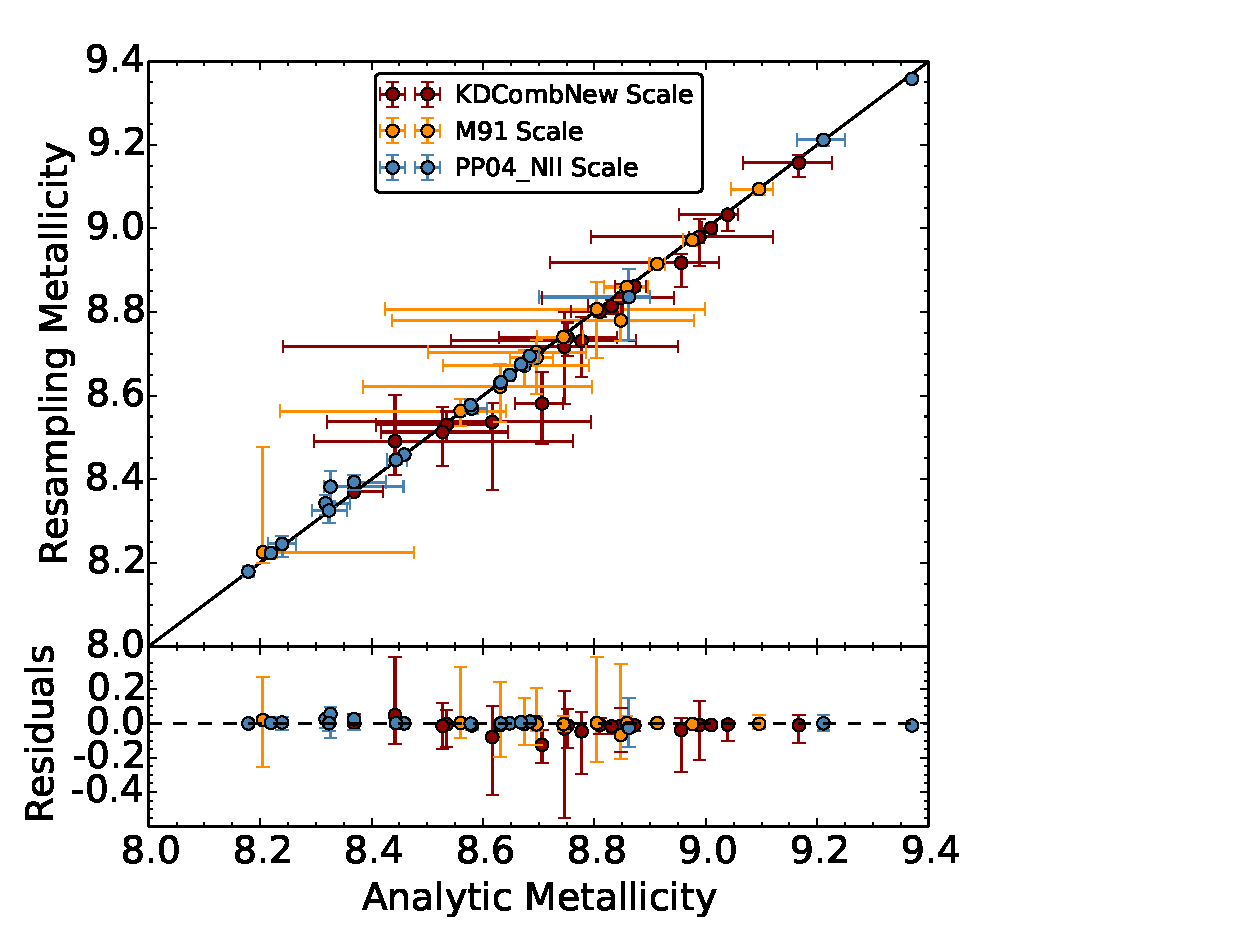
\includegraphics[trim = 10mm 0mm 10mm 0mm, clip]{abcomparison6.eps}
  \includegraphics[width=0.95\columnwidth]{exampledata_n2000_PP04_O3N2_1KDE.pdf}
   \caption{\textbf{FINISH}}
\label{fig:KDE}
\end{figure}
Lastly, we enable the user to obtain a distribution Kernel Density if the \verb=sklearn= is available. The Kernel Density of the distribution is then calculated via  \emph{KD Tree} with a top-hat function, as explained in the sklearn package documentation \footnote{\url{http://scikit-learn.org/stable/modules/density.html}}. The results will then show both a histogram, with $N_\mathrm{bins}$ chosen via Knuth's method, as well as the distribution Kernel Density, as shown in Figure~\ref{fig:KDE}.


\begin{figure}[ht!]
%  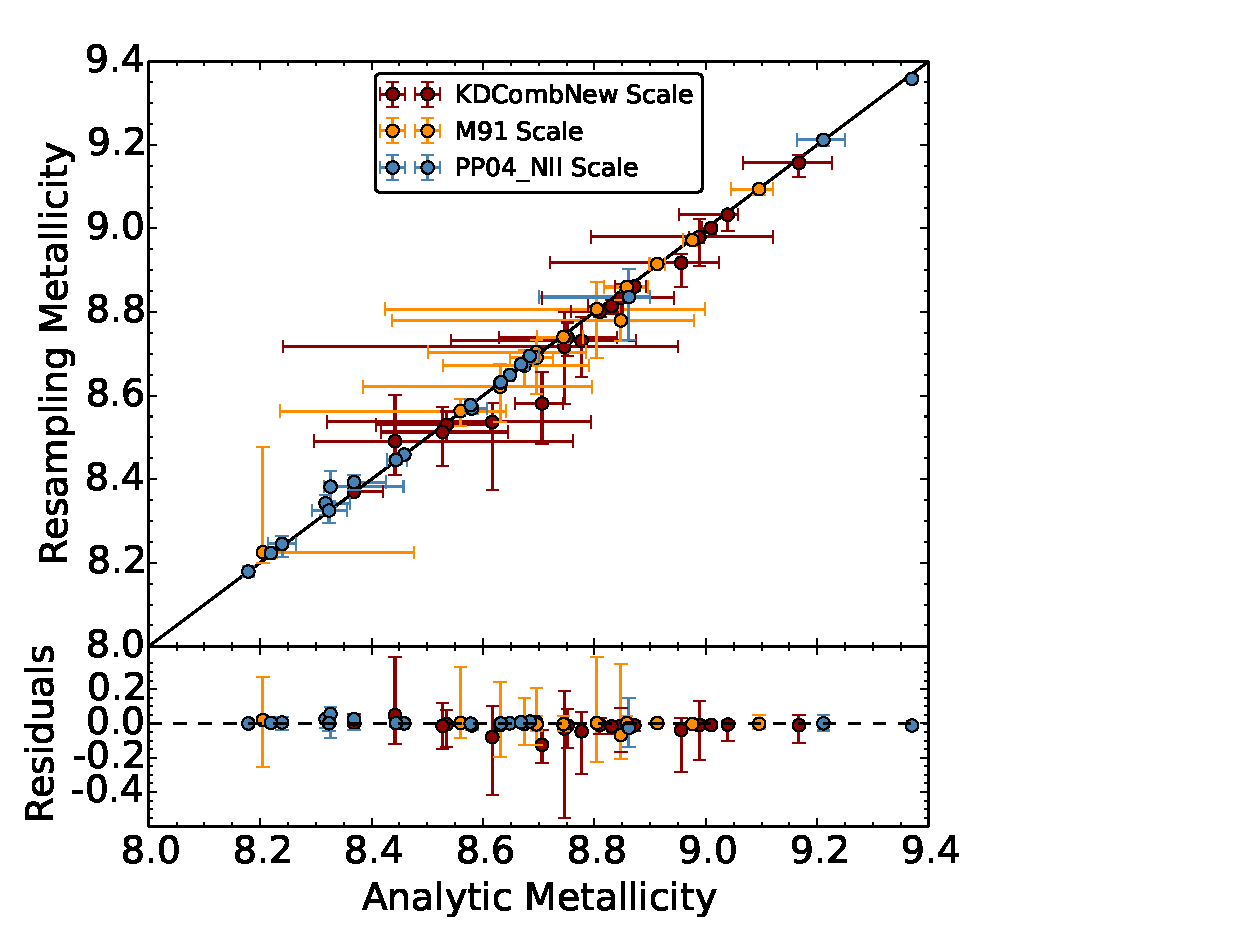
\includegraphics[trim = 10mm 0mm 10mm 0mm, clip]{abcomparison6.eps}
  \includegraphics[width=0.95\columnwidth]{exampledata_boxplot2000_m1.pdf}
   \caption{\textbf{FINISH}}
 \label{boxplot}
\end{figure}

The boxplot summarizes the resut from each scale the user chooses to calculate. For each scale a box is shown, and the box height represents the 25\% percentile of the \oxab~ distribution. Inside the box a black line represents the distribution median, the bars represent the maximum and minimum value of the distribution, excluding outliers, and the outliers are plotted as circles, and are defined as all datapoints more than one and a half times the length of the box from either end of the box (or 1.5xIQR, where IQR is the the \emph{interquartile range}). The solar oxigen aboundance is indicated in this plot for comparison: a gray box shows a range of estimated values for solar oxigen aboundances, from \oxab=8.69 \citep{Asplund09} to \oxab=8.76 \citep{Caffau11}. 
Notice that only the diagnostics requested by the user have a slot in the plot (in the example in Figure~\ref{fig:KDE} the computed scales are M91, the PP04 scales, and the KD02 scales. However these slot exists on the plot whether the diagnostic can be produced or not, i.e. if the input lines to not allow a requested scale to be calculated an empty coulmn will be generated in this plot in correspondence of said metallicity scale.\

%Using a bin size of $\sqrt{N}$ was recommended, but this proved to be slightly over-fitting, and after a number of tests, we found $2* \sqrt[3]{N}$ to be appropriate for most cases.

% While the histograms at sufficiently high $N$, where $N$ is the total number of iterations, yielded single peaked results, at lower $N$ there were occasional multiple peaks resulting from a non-smooth gaussian being sampled. In selecting the value of $N$, we found that around $N=20,000$ the KS tests showed the same distributions as larger sized samples, i.e. that the results converged ({\bf FED CHECK MY WORDING!}). 









\section{Comparison to prior uncertainty computation and other works }\label{comp_sec}


A previous method for determining the uncertainty in the oxygen abundance (as used in \citealt{modjaz08_Z,kewley10,rupke10,modjaz11}) was an \emph{analytic} approach of propagating the emission-line flux uncertainties: it found the maximum and minimum abundances via maximizing and minimizing, respectively, the various line ratios by adding/subtracting to the measured line values their uncertainties. For comparison we computed the metallicities and their errors in both ways (both analytic and using our current MC resampling method) for 3 representative scales. We plot our results and the residuals in Fig.\ref{comp_anal_MC}, which shows a number of important points: i) The metallicity reported as the 50th percentile of the metallicity parameter distribution from the MC resampling method is completely consistent with the analytically derived metallicity -  well within the respective error bars - and thus, the prior published results still stand (unsurprisingly, since our code, aside for the calculation of the confidence interval, uses the same algorithms developed for IDLKD02). ii) The MC resampling method has smaller error bars than the analytic method, especially for the scales of M91 and KD02. This is easily understandable, since the analytic method assumes the worst-case-scenario, as it basically yields 2 metallicity parameter draws (the "minimum" and "maximum") which are in the tail of the full metallicity probability distribution. However, the MC resampling method is the more appropriate method as it empirically characterizes the full parameter estimation distribution.
%assumes that \textbf{all} emission line measurement have been drawn from the 68\% tail of the error distribution and 

\begin{figure}[ht!]
%  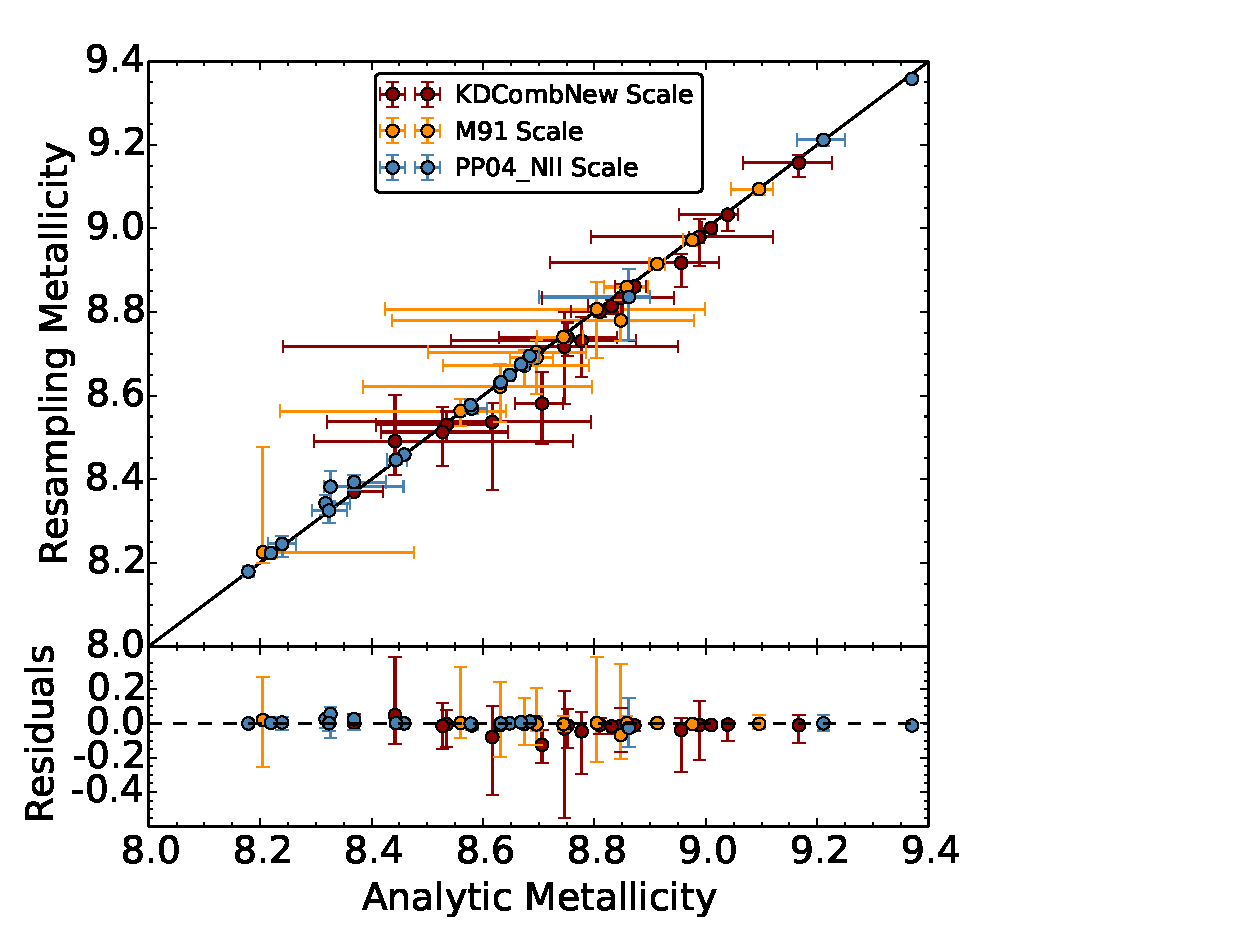
\includegraphics[trim = 10mm 0mm 10mm 0mm, clip]{abcomparison6.eps}
  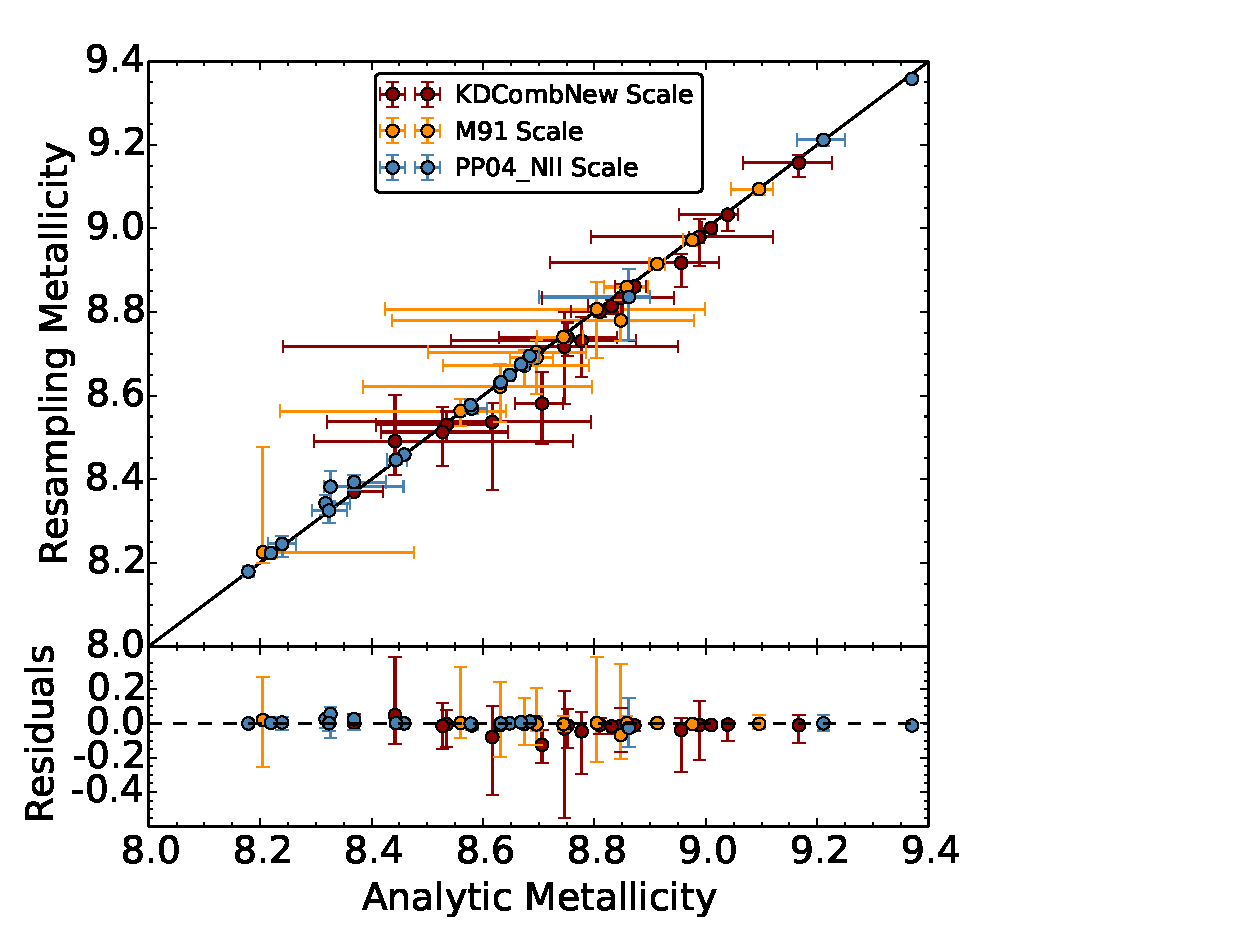
\includegraphics[width=1.2\columnwidth]{abcomparison6.eps}
   \caption{\textbf{FINISH}.Comparison of metallicity estimation between the analytic method and our Monte Carlo resampling method (top) and their residuals (bottom) for 3 different metallicity scales. Flux measurements come from 19 galaxies previously measured in \citet{modjaz11}. To add asymmetric errors in quadrature we use $residual_{min}=\sqrt {x_{max}^2 + y_{min}^2}$ and $residual_{max}=\sqrt {x_{min}^2 + y_{max}^2}$}
 \label{comp_anal_MC}
\end{figure}




%Although the flux probability distribution function is assumed to be symmetric, the metallicity errors are asymmetric because they are derived from the log of minimized and maximized flux ratios.
%Rupke: Errors were propagated primarily using analytic expressions, but for abundance and gradient errors we employed Monte Carlo methods.

\subsection{Comparison with other works}

%Here we perform a literature review of both 


The field of SN host metallicity studies has been rapidly developing as these kinds of studies may be crucial avenues for constraining the progenitor systems of different kinds of explosions - however, a few of the works do not even compute errors and others not show how they compute their statistical errors or  (e.g., \citet{anderson10,leloudas11,sanders12,leloudas14}). While \citet{sanders12} compute the line flux errors from a Markov-Chain Monte Carlo fitting of a gaussian to the emission lines, they only mention in passing that they propagate the line flux uncertainties into the metallicity measurements, but do not describe how {\bf this is a little harsh, right? i think mentioning it without explaining is generally the standard for iid errors -> Maryam: " How would you rephrase it then? " }.

%by propagation of the uncertainties in the line flux measurements
%and the 0.07 dex diagnostic systematic error.
%( line flux errors from MCMC fitting of a gaussian to emission lines)

In contrast, the general metallicity field has considered in detail how to estimate the uncertainties in measured metallicities- however, none of those codes are open-source and many of them are for specific scales which were chosen by the authors:  \citet{moustakas10} also use MC resampling to estimate the metallicity uncertainties (in their case using 500 trials which seems to lead to a Gaussian distribution) but only do this for two scale, KK04 and \citet{pilyugin05}. For computing the metallicities of the SDSS star forming galaxies, \citet{tremonti04} fit a combination of stellar population synthesis and CLOUDY ({\bf citation}) photoionization models to the observed strong emission lines [OII], $H\beta$, [OIII], $H\alpha$, NII and SII and report the median of the metallicity likelihood distribution as the metallicity estimate, with the width of the distribution giving the 1 $\sigma$ (Gaussian) error. However, this is constitutes their own scale (the T04 scale).

In the last stages of preparing this manuscript \citet{blanc15} was published.  \citet{blanc15} employ Bayesian inference for doing something similar to \citet{tremonti04} - they use Bayesian inference to derive the joint and marginalized posterior probability density functions for metallicity $Z$ and ionization parameter $q$ given a set of observed line fluxes and an input photoionization model. They provide a publicly available IDL implementation of their method named $IZI$ (inferring metallicities (Z) and ionization parameters) on the author's website.


\section{Conclusions}\label{comp_sec}

 \textbf{FINISH}. We hope that this open-access code will be used in many different fields where gas-phase metallicities are important, including in the emerging field of SN and GRB host galaxies, where either it is not described how they got  or no error bars are computed (e.g., \citealt{lunnan14}). GIven its public-access nature, the users are free to include any new metallicity diagnostics, e.g., that suggested by \citet{dopita13}.

\acknowledgements
M. Modjaz is supported in parts by the NSF CAREER award AST-1352405 and by NSF award AST-1413260. FBB is supported by a \emph{James Arthur Fellowship} at the NYU-Center for Cosmology and Particle Physics. Some plots are  produced with public code DOI:10.5281/zenodo.15419 available at \url{https://github.com/fedhere/residuals_pylab}.
 This research made use of NASA Astrophysics Data
System; the NASA/IPAC Extragalactic Database (NED), which
is operated by the Jet Propulsion Laboratory, California Institute
of Technology, under contract with the National Aeronautics
and Space Administration.



%\epsscale{1.0}
%\begin{center}
%\csvautotabular{table1.csv}
%\label{t1}
%\caption{Comparison of M-M method with MC method}
%\end{center}
%\end{figure*}



%%%%%%%%%%%%%%%%%%%%%%%%%%%%%%%%%%%%%%%%%%%
%%\clearpage
%%%%%%%%%%%%%%%% BIBLIOGRAPHY  %%%%%%%%%%%%%%%%%%%%%%%% 
\bibliographystyle{apj}
%\bibliography{refs}
\bibliography{refs}

\appendix

\section{Minimum Code validation}
\textbf{WORK WITH FED - and any other code specific things}
\end{document}


@INPROCEEDINGS{astroML,
  author={{Vanderplas}, J.T. and {Connolly}, A.J.
          and {Ivezi{\'c}}, {\v Z}. and {Gray}, A.},
  booktitle={Conference on Intelligent Data Understanding (CIDU)},
  title={Introduction to astroML: Machine learning for astrophysics},
  month={oct.},
  pages={47 -54},
  doi={10.1109/CIDU.2012.6382200},
  year={2012}
}}

@BOOK{astroMLText,
  title={Statistics, Data Mining and Machine Learning in Astronomy},
  author={{Ivezi{\'c}}, {\v Z}. and {Connolly}, A.J.
          and {Vanderplas}, J.T. and {Gray}, A.},
  publisher={Princeton University Press},
  location={Princeton, NJ},
  year={2014}
}

%,page]{appendix}
%\usepackage{amsmath}
%\usepackage{amssymb}
%\usepackage{verbatim}
%\usepackage{graphicx}
%\usepackage{epsfig}
%\usepackage{morefloats}
%\usepackage{float}
%\usepackage{lipsum}
%\usepackage{subfigure}
%\usepackage{longtable}
%\usepackage{lipsum} 
%\usepackage{rotating}
%\usepackage{wasysym}

\begin{document}
\title{Monte Carlo Method for Calculating Uncertainty in Oxygen Abundance from Strong-Line Flux Measurements}

\author{Author order to be determined: Maryam Modjaz\altaffilmark{1}, Federica B. Bianco\altaffilmark{1}, Seung Man Oh\altaffilmark{1,2}, David Fierroz\altaffilmark{1}, Yuqian Liu\altaffilmark{1}, Lisa Kewley\altaffilmark{3,4}}
\altaffiltext{1}{Center for Cosmology and Particle Physics, New York University, 4 Washington Place, New York, NY 10003, USA}
 \altaffiltext{2}{NYU Abu Dhabi PO Box 129188 Abu Dhabi, UAE}
 \altaffiltext{3}{Australian National University, Research School for Astronomy \& Astrophysics, Mount Stromlo Observatory, Cotter Road, Weston, ACT 2611, Australia }
 \altaffiltext{4}{ Institute of Astronomy, University of Hawaii, 2680 Woodlawn Drive, Honolulu, HI 96822, USA}
 
 
\begin{abstract}
\textbf{MODIFY \& FINALIZE AT THE END:} We present an open-source Python code for the determination of the strong-emission-line estimators of oxygen abundance in the standard scales, based on the original IDL-code in \citet{kewley02}. The standard strong line Metallicity scales and diagnostics \text{IMPROVE} have been used to estimate metal abundance through emission line ratios. Here we introduce a Monte Carlo resampling of these methods in order to better characterize an oxygen abundance confidence region.  We output median values, 16th and 84th percentile confidence regions, for various standard metallicity diagnostics, and, when possible, for reddening E(B-V). We produce Monte Carlo parameter distributions for the oxygen abundance and when possible for reddening E(B-V). We test our code on emission lines measurements from a sample of galaxies ($z<0.15$) and compare our metallicity results with those from previous methods. We show that our metallicity estimates are consistent with previous methods but yields smaller uncertainties. The code is open source and can be found at www.github.com/nyusngroup/ \textbf{
(add repo and DOI)}.
\end{abstract}
 
\section{Introduction}
The low quantity of carbon, oxygen, nitrogen, sulfur and iron among other elements provide a splash of color to the otherwise dominating greyscape of hydrogen and helium in the stars and gas of galaxies. Nevertheless, even the minute presence of heavy elements (all elements heavier than H and He, also called metals or collectively metallicity) is important for many areas of astrophysics. For example, \citet{johnson12} suggest that if it was not for the relatively high metallicity level in our Solar System, planet formation may not have been possible. With $Z$ representing the mass fraction of metals, for our own Sun the value is measured to be  Z=0.0153 \citep{chaffau11}, though there are others who suggest a lower solar metallicity of $Z=0.0134$ in particular because of oxygen \citep{asplund09_rev,grevesse10}\footnote{Note that these abundances refer to the current abundances in the sun, which are lower than the value with which the sun was formed 4.56 Gyr ago, since diffusion at the bottom of the convection zone has decreased metallicity over time \citep{grevesse10}.}. Furthermore, when properly observed and estimated, metallicity measurements of galaxies can tightly constrain models of galaxy formation and evolution (e.g., \citealt{kewley08} and references therein), tas well as shed light on the metallicity dependence and production conditions for different types of SNe and long-duration GRBs (e.g., \citealt{modjaz08_Z,levesque10_grbhosts,anderson10,modjaz11,kelly12,sanders12,lunnan14,leloudas14}), to just name a few examples.

%chaffau Z=0.0209 12+log=O/H) = 8.76�0.07 i
%Small variations in chemical abundance can often be critical indicators for stellar and galactic properties like age and activity.
%Metals are produced in the cores of stars during their fusion lifecycle but also during the extreme conditions of stellar explosions. For example, the majority of iron comes from thermonuclear explosions (SN Ia) while nearly all of oxygen is the result of core collapse (SN Ib, Ic, \& II). Since new stars are born from the clouds these explosions produce, metallicity will increase with each passing generation. Stars like our Sun, which are results of multiple generations of star formation, are often found in the more active parts of the galaxy, such as the disk, and are referred to as Population I stars. Population I stars have higher metallicity than older Population II stars, which are also present in the disk but are the exclusive members of the low activity galactic halo. Population III stars would be first generation stars with zero metallicity, but have yet to be observed.
%Besides age, metallicity also influences stellar temperature. Metals are more effective at absorbing energy coming from the interior of the star in the stellar atmosphere so their presence increases the stellar opacity. With greater absorption and opacity the radius expands to a size larger than it would be without metals and this larger size results in a cooler effective temperature. While metallicity can help indicate age or activity it's temperature and density dependencies require parameterization to properly be estimated.

However, for almost all astronomical objects, metallicity cannot be measured directly. The oxygen abundance in the gas-phase is the canonical choice of metallicity indicator for interstellar medium (ISM) studies, since oxygen is the most abundant metal and only weakly depleted onto dust grains (in contrast to refractory elements such as Mg, Si, Fe, with Fe being depleted by more than a factor of 10 in Orion; see \citealt{simondiaz11-orion}). The oxygen abundance\footnote{We note that in many cases in the literature, including here, the terms metallicity and oxygen abundance are used interchangeably.} is expressed as  $12 + \log_{10}(\frac{O}{H})$, where $O$ and $H$ represent the number of Oxygen and Hydrogen atoms, respectively. Importantly, oxygen exhibits very strong nebular lines in the optical wavelength range of HII regions (e.g., \citealt{pagel79,osterbrock89,tremonti04}), and thus, many different diagnostic techniques, relying on different lines, have been developed (e.g., \citealt{kewley02,pettini04,kobulnicky04,kewley08}), which are discussed in the next section.

\subsection{The different oxygen abundance diagnostics}
Here we present a brief overview of the various observational methods for measuring the gas-phase oxygen abundance - however, for a full discussion with all the caveats we encourage the reader to see reviews by e.g. \citet{stasinska02,kewley08,moustakas10,stasinska10,dopita13,blanc15}.
The so-called ``classical'' way to estimate the oxygen abundance is the electron temperature ($T_e$) method, which estimates the electron temperature and density of the nebula using a number of oxygen lines with different ionization states, including the auroral [OIII] $\lambda$4363 line, to then directly estimate the OII and OIII abundances to obtain the total oxygen abundance, after correcting for the unseen stages of ionization. However, the auroral [OIII] $\lambda$4363 line is very weak, even in low-metallicity environments, and saturates at higher metallicity (since at higher metallicities the cooling is dominated by the Oxygen NIR fine structure lines) $-$ thus, other methods had to be developed that use other, stronger lines, in the spectra of HII regions. These are called strong-line methods and are the subject of this manuscript. Strong-line methods can be categorized into two types: theoretical methods, that rely on calibrating various observed line ratios using photoionization methods (basically theoretically simulating HII regions, using stellar model atmospheres, stellar population synthesis and photoionization models) and empirical ones that calibrate various observed strong line ratios using observed $T_e$-based metallicities. While historically there have been large systematic offsets between the $T_e$ method and the strong line methods, \citet{dopita13} demonstrated that the $T_e$ method gives the same results as the strong line methods, if the energy distribution of the electrons in the HII regions is assumed to not be a simple Maxwell-Boltzmann distribution (as assumed in prior works), but a more realistic $\kappa$ distribution, as observed in solar system astrophysical plasma. They also find that the effect of the $\kappa$ distribution on the strong-line methods is minor.


For the theoretical strong-line method, one ratio that is commonly used to determine the metallicity of galaxies is ([OII] $\lambda 3727$ $+$ [OIII] $\lambda 4959,\lambda 5007$)$/$H$_\beta$ \citep{pagel79} and is referred to as R23. The drawback of this method is that it is double-valued with metallicity, and thus other line ratios need to be used to break the degeneracy between the high values ("upper branch") and the low values ("lower branch") of the R23 metallicities. Furthermore, \citet{kewley02} showed the importance of ionization parameter, which can be physically understood to correspond to the maximum velocity of an ionized front that can be driven by the local radiation field of hot massive stars that are ionizing the ISM gas. This ionization parameter needs to be taken into account in the various strong-line methods, as HII regions at the same metallicity but with different ionization parameters produce different line strengths. Calibrations of R23 by \citet{mcgaugh91} (hereafter M91) and by \citet{kewley02} (hereafter KD02) use different theoretical photoionization models and take the ionization parameter into account, while other calibrations such as of \citet{zaritsky94} (hereafter Z94) do not. Thus, Z94 is mostly valid for only metal-rich galaxies.  M91 and KD02 use an iterative process to break the R23 degeneracy  (KD02 uses different ratios [NII]$/$[OII] and [NII]$/$H$_\alpha$) and to also constrain the ionization parameter $q$ in order to arrive at the metallicity estimate.

%The most direct way to estimate metallicity in spectra is to measure line fluxes absorbed or emitted by metals and non-metals. While iron lines may be present in stellar spectra, iron is less commonly found in gaseous nebulae than oxygen is. Not only is oxygen more abundant but it emits several strong lines ([OI] $\lambda 6300$, [OII] $\lambda 3727,7318,7324$, [OIII] $\lambda 4363, 4959, 5007$) visible at optical wavelengths that can also be used to quantify temperature and density. For this reason 
%While the ratio of oxygen to hydrogen line flux correlate with metallicity, the ratio of two [OIII] lines, one auroral $\lambda 4363$ and the other an excitation line at $\lambda 5007$ can be used to determine what is called the Ionization Correction Factor (ICF) (Kewley \& Dopita 2002).
As to empirical strong-line methods, the most commonly used one is that by \citet{pettini04} (hereafter PP04). PP04 used HII regions with $T_e$-based metallicities to derive empirical fits to strong-line ratios, and introduce the line ratios of ([NII]$/$H$_\alpha$ (N2) and ([OIII]$/$H$_\beta$)$/$([NII]$/$H$_\alpha$ (O2N2) as metallicity diagnostics. Since PP04-N2 employs two closely spaced lines (Halpha and NII), which are not affected by stellar absorption, nor uncertain reddening, and are easily observed in one simple spectroscopic setup, it has become an often-used scale for at least low-z SN host galaxy studies (e.g. see metal-analysis by e.g,. \citealt{sanders12,modjaz12_proc,leloudas14}). However, it is important to remember that this scale has a number of short-comings: it does not take into account the impact of the ionization parameter, it was initially derived based on only 137 extragalactic HII regions, and the nitrogen emission line employed saturates at high metallicity (\textbf{CHECK!}), and thus this method may not be well-suited for high-metallicity galaxies. An updated calibration by \citet{marino13} based on many more Te-based metallicities (almost three time larger that that of PP04) derives a significantly shallower slope between O3N2 index and oxygen abundance than the PP04 calibration.


As it can be seen, each scale has different advantages and disadvantages and should be used in different metallicity regimes (see detailed discussion in e.g.,  \citealt{kewley02,stasinska02,kewley08,moustakas10,dopita13,blanc15}). Thus, this open-source code outputs the oxygen abundance in the main 6 metallicity scales (for which the KD02 diagnostic has four outputs and the PP04 diagnostic has two outputs). While there is a long-standing debate about which diagnostic to use, as there are systematic metallicity offsets between different methods (recombination lines vs.  strong-line method vs. ``direct'' $T_e$ method, see the above sources), \emph{\bf the relative metallicity trends can be considered robust, if the analysis is performed self-consistently in the same scale, and trends are seen across different scales \citep{kewley08,moustakas10}}. Note however, that while there are conversion values between different scales \citep{kewley08}, they apply for large data sets, since those conversion values were derived based on ten thousands of SDSS galaxies, and thus should be used with caution (or not at all) for smaller samples. In addition, one should note that there is a debate about the value of the solar oxygen abundance \citep{asplund09_rev,chaffau11}, such that the absolute oxygen calibration is still uncertain.




Here we introduce the open-source python code "". pro .. In \S~\ref{method_sec} we describe our method, the input and output values of the code. In \S~\ref{comp_sec}, we compare our method of obtaining abundance uncertainties to previous methods in the literature. 
%\begin{figure}[H]
%\epsscale{1.0} 
%\begin{center}
%\includegraphics[width=0.89\columnwidth]{fig1.png} 
%\caption{Example of a sampled Gaussian. 50,000 points from a Gaussian distribution were selected in this case}
%\label{f1}
%\end{center}
%\end{figure}


\section{Description of Metallicity code}\label{method_sec}


\begin{figure*}[!HT]
%\epsscale{0.6}
\begin{center}
\centerline{
\includegraphics[width=0.95\columnwidth]{exampledata_n2000_KD02comb_1.pdf}
%exampledata_n50000_KD02comb_updated_1.ps}
\includegraphics[width=0.95\columnwidth]{exampledata_n2000_PP04_O3N2_1.pdf}}
%exampledata_n50000_PP04_O3N2_1.ps}
\vspace{0.2in}
\centerline{
\includegraphics[width=0.95\columnwidth]{exampledata_n2000_M91_1.pdf}
% exampledata_n50000_M91_1.ps}
\includegraphics[width=0.95\columnwidth]{exampledata_n20000_E(B-V)_1.pdf}}
%exampledata_n50000_EBV_1.ps}

\caption{WILL UPDATE WITH NEW FIGURES BASED ON A PUBLISHED SN WITH SIGNFICANT E(B-V) AND WRITE MORE TEXT. Metallicity and reddening ($E(B-V)$) parameter distributions based on example data (namely, emission line data of the HII regions at the position of SN~2008D, published in \citet{modjaz11}, based on $N$=20,0000 samples. The median value is shown with the dashed lines, while the 16th till 84th confidence region is shaded in tan color. The shown metallicity scales are  by \citet{kewley02}, updated by \citet{kewley08} (KD02combupdated), \citet{pettini04}, using OIII and NII  (PP04-O3N2) and \citet{mcgaugh91} (M91). These are the same plots that are outputted by the code, which produces such plots for all scales (namely those of s\textbf{LIST THEM ALL}). The legend also includes the ID number of }
 \label{metallicity_distribution}
\end{center}
\vspace{-0.5in}
\end{figure*}


For computing oxygen abundances, we use the iterative code by \citet{kewley02}, which has been updated in \citet{kewley08} and reflects .. \textbf{LISA: YOUR INPUT HERE:what is the update??} which was initially written in IDL.  We translated the code into python, added the new feature of obtaining uncertainties on the metallicity outputs via Monte Carlo resampling, and made it open source via github, as we explain below.

We assume that the observed emission lines to be used to indicate metallicity originate in HII regions and are not due to non-thermal excitation by e.g., AGN or interstellar shocks from SNe or stellar winds.  Tests to exclude data contaminated by such non-thermal sources should be executed using the recommended line ratios by e.g., \citealt{baldwin81,kauffmann03,kewley06_sdss} prior to running this code. Furthermore these lines should have all the correct calibration (at least correct relative calibration) and should have a signal-to-noise ratio (S/N) of at least 3. The latter is important for the success of the Monte Carlo resampling technique as described below.

\subsection{Input and Output of code}
Emission line flux values are fed into our Python implementation as in the original IDL code by \citet{kewley02}, hereafter referred to as IDLKD02. The inputs are emission line flux values and their uncertainties for the following lines: H$\alpha$, H$\beta$, [OI] 6300, [OII] 3727, [OIII] 4959, [OIII] 5007, [NII] 6584, [SII] 6717, [SII] 6731, SIII 9532, and SIII 9096 \textbf{CHECK AT THE END WITH CODE!} and their uncertainties (consult the README.md in the github repository for details about the input format). If the fluxes for the specified lines are not available, the entry is left to 0 \textbf{FED: we should do NaN!???} and the outputted oxygen abundance scales will be in only metallicity scales that use the provided line fluxes. As part of the code, the inputted line fluxes are corrected for reddening by using the observed Balmer decrement, for which H$\alpha$ and  H$\beta$ flux values need to be provided. We assume case B recombination, and thus the standard value of 2.86 as the
intrinsic H$\alpha$/H$\beta$ ratio \citep{osterbrock89}, and apply the standard Galactic reddening law with $R_V$ = 3.1 \citep{cardelli89}. However, the user can choose other extinction laws and $R_V$ values, if desired, given the code's open-source nature.

While other parameters, such as the ionization parameter $q$ and the electron density (using the SiII lines) are computed as long as the necessary lines are provided, they are not outputted in the current version of our code $-$ however, the reader is welcome to easily modify the code to suite their needs, given it's an open-source code.

As output, we obtain metallicity values and their uncertainties in the following calibrations, as discussed in detail in \citet{kewley02,kewley08}: \citet{kewley02}(KD02, for the 4 following computations: R23, using the NIIOII ratio, using the NII/Halpha ratio, and a combined method that uses the optimal method given the input line fluxes), \citet{mcgaugh91} (M91), \citet{zaritsky94} (Z94), \citet{pilyugin01} (P01), \citet{denicolo02} (D02), 
\citet{pettini04} (2 computations: PP04-N2, PP04-O3N2) \textbf{CHECK WITH FINAL CODE - ALSO CHECK whether P01 is P01 or P05 by looking at the code}. If the line fluxes necessary for specific scales are not provided, the output  metallicities will default to -1, if the errors in he measurements are not provided, the code will specify that it cannot create a measurement distribution and determine a confidence interval.



\subsection{Computing Uncertainties}
The novel aspect of our work is that for every set of input line measurements we introduce a Monte Carlo (MC) resampling method to obtain iterations via random sampling within the measurement errors, and thus we obtain a robust result for error estimation (e.g., \citealt{efron79,hastie09,andrae10}). 

Given a data set with error bars from which certain parameters are estimated, Monte Carlo resampling generates synthetic data samples drawing from a given distribution. 
Here we draw synthetic data from a Gaussian distribution centered on each measured line flux value, with standard deviation corresponding to the measurement error. The implicit assumption is made, of course, that the line flux error is Gaussian distributed in nature\footnote{The user may wish to provides their own probability distribution for the emission line uncertainties, and easily modify the code to suite their needs.}. 

% FED: because we vectorize, we actually do not do this sample by sample so we cannot say ``Every iteration''
For each metallicity scale, for each of $N$  values chosen randomely within the relevant emission line distributions we run the calculations that derives the metallicity.
This effectively simulates conducting multiple experiments when repeating observations is impractical or impossible, as in the case of the emission line flux data, and thus generates alternative data sets. 
%FED redundant: We generated $N$ Monte Carlo flux samples for each emission line, and calculated the metallicity for each set of line fluxes. 
The sample size $N$ is set by the user, and one should expect an appropriate value of $N$ to be a few 1000s, depending on the metallicity scale chosen and measurement errors (for example  $N=2,000$ is determined to be sufficient for our example data, as shown below, and we provide tools to assure the sample size is sufficiently large). 
%FED: note that 2000 is ok for our sample but it does not need to be! it depends on the error size, and the shape of the distribution, so it depends on the input. if for example the distribution 
% , FED: because we vectorize, we actually do not do this sample by sample, so we cannot say ``At the end of $N$ iterations''
A parameter estimate distribution of oxygen abundance is generated for each scale, the metallicity and its confidence region are calculated,
%We bin to visualize, but we calculate percentiles on the actual distribution
and the results are bunned abd visualized in a histogram (see below)\footnote{However, note this method is a conservative approach, since it overestimates the intrinsic metallicity uncertainty, as we are centering this error distribution on the measured values instead of the (unknown) true values \citep{andrae10}.
%FED i do not know what that means. i would think that this method is NOT conservative on account of that!
}. This is done for each scale the user chooses to calculate. The fiftieth (50\%) percentile, i.e.  the median, is reported as the measuredtrue metallicity value, and the 16th and 84th percentiles of the distribution as its confidence region. %FED redundant? The output of our code includes the oxygen abundance measurements plus confidence regions in all scales, as well as plots of the distributions of the oxygen abundance value in all scales. 

This MC resampling approach takes into account the impact of the uncertain reddening (due to the uncertainties in the measurement of the 
H$\alpha$ and H$\beta$ fluxes), when the option for de-reddened metallicities is chosen. Since for each iteration, a new reddening value is calculated based on the resampled H$\alpha$ and H$\beta$ fluxes, which is used to compute the de-reddened metallicity value, the derived distribution of metallicity values takes into account the uncertain redding. As part of the output, a probability distribution plot for E(B-V) is provided (see last plot in figure~\ref{metallicity_distribution}, along with confidence intervals derived using the same method as for the metallicity measurements. If either H$\alpha$ or H$\beta$ flux is not provided, then no reddening correction can be applied and the computed metallicity will not be  reddening-corrected and the E(B-V) output will be set to zero.

Figure \ref{metallicity_distribution} shows the metallicity estimate distribution for 3 representative scales, and for the reddening parameter E(B-V) - similar plots that are outputted by our code for all scales as listed above (not all shown here). Although the input distributions are Gaussian, the metallicity distributions 
%FED: in log space they are NEVER gonna be gaussian so not ``rarely are'',
are not, for two reasons: first, since the metallicities are computed based on log values of line flux ratios, symmetric error bars in linear space will translate into asymmetric error bars in log space; and second, some metallicity computations are non-linear, and (especially those that include $R_{23}$) sometimes bimodal since they choose upper vs lower branch to break degeneracy.

Since the metallicity distributions are rarely Gaussian, the percentiles we report cannot be expressed in terms of $\sigma$ values. In determining the confidence region intervals for asymmetric and multi-modal distributions, there are broadly three approaches (e.g., \citealt{andrae10}): choosing a symmetric interval, the shortest interval,  or a ``central'' interval.  With the "central" method we determined the  confidence interval by choosing the left and right boundaries such that the region outside the confidence interval each equally contains $16\%$ of the total distribution - in analogy to the one-sigma-interval of the Gaussian distribution. This ensures that the algorithm finds the proper boundaries even for asymmetric, non-Gaussian, distributions, (i.e., multimodal likelihood distributions) and in the case of multiple peaks. 

In summary, the output for the measured value corresponds to the fiftieth (50\%) percentile, while the lower error bar corresponds to the 50$^{th}$-16$^{th}$ percentile and the upper error bar corresponds to 84$^{th}$-50$^{th}$ of the metallicity parameter estimate distribution. However, we urge that the reader always inspect the appropriate metallicity distribution plots, which are also outputted, to check for themselves whether the outputted median and confidence regions properly represent the full metallicity distribution (see Section~\ref{visz}).

We note that our code  does not output the \emph{systematic} uncertainty of each scale, which are e.g., $\sim$ 0.07 dex (or 0.14 dex \textbf{CHECK}) for PP04-O2N2.  Thus systematic errors can be as large, if not larger, than the statistical errors, however, if all metallicity measurements are in the \emph{same} scale and only \emph{relative} comparisons are made, then the systematic error does not have any impact (by definition!). The distributions for the D02 scale include the uncertainty in the fit parameters: the oxygen aboundance in this scale is generated as \oxab~=~$9.12~\pm 0.05 + (0.73~\pm 0.10)~\mathrm{NII}$, as published in  \citet{denicolo02}. The parameter fit are generated as the sum of the nominal parameter (9.12 and 0.73) and a Gaussianly distributed random value centered on zero, and within a standard deviation of 0.05 and 0.10, respectively.

%However, the
%relative metallicity difference measured between a given pair
%of galaxies in different diagnostics is consistent with an rms
%scatter typically ?0.07 dex, and 0.15 dex between the most
%discrepant diagnostics (Kewley&Ellison 2008).


%from Kewley & Ellison08: The cause of the metallicity calibration discrepancies remains unclear. The discrepancy has been attributed to either an unknown problem with the photoionization models (Kennicutt et al. 2003) or temperature gradients or fluctuations that may cause metallicities based on the electron temperature method to underestimate the true metallicities (Stasin�ska 2002, 2005; Bresolin 2006). Until this discrepancy is resolved, the absolute metallicity scale is uncertain.

\subsubsection{Visual diagnostics}\label{visz}
In order for the user to check the validity of a measurement, and to better understand the distribution, we provide two visualizations: for each metallicity scale calculated, for each input set, we generate a histogram of the output distribution (Figure \ref{metallicity_distribution} and \ref{fig:KDE}), and for each set of input line we generate a \emph{box-and-whiskers} plot (herehance \emph{boxplot}, for short) summarizing the result of all scales calculated (Figure \ref{boxplot}). 

Choosing the binning size for a histogram is not a trivial task.  \citet{hogg08} describes various data analysis recipes for selecting a histogram bin size. Too many bins will result in many empty bins and an ``over-fit'' histogram, while too few bins may miss features of the distribution. 
By default, we use \emph{Knuth's Method} to choose the number of bins $N_\mathrm{bins}$ for each histogram. Knuth's method  optimizes  a Bayesian fitness function across fixed-width bins \citep{Knuth06}. Additionally, however, we enable a number of binning options from which the user can choose, including: 
the square root of the number of bins, \emph{Rice rule} ($N_\mathrm{bins}~=~2\sqrt[3]{N}$, e.g., \citealt{hastie09}), 
\emph{Doane's formula} ($N_\mathrm{bins}~=~1 + \mathrm{log}_2{N} + \mathrm{log}_2\left(1 + \mathrm{Kurt}\sqrt{(N / 6)}\right)$, where Kurt is the third standardized moment of the distribution \citealt{Doane76}\footnote{\citet{Doane76} attempted to address the issue of finding the proper number of bins for the histogram of a skewed distribution. Several version of the so-called Doane's formula can be found in the literature. Our formula can, for example, be found in \citealt{Pharmacokinetic}}), and the full Bayesian solution, known as Bayesian Blocks, which optimizes a fitness function across an arbitrary configuration of bins, such that the bins are of variable size \citep{scargle13}. The implementation of the latter method requires the \verb=astroML= python package to be installed on the user's system (\citealt{astroml}\footnote{\url{https://github.com/astroML/astroML}}). If the \verb=astroML= package is not found, the code will default to Knuth's Rule. 

As mentioned, Knuth's method implies an optimization. In cases in which the convergence of this minimization takes too long (or if the number of bins after the minimization is  $N_\mathrm{bins}/\sqrt{N} > 5$ or $N_\mathrm{bins}/\sqrt{N} < 1/3$) the code will revert to Rice rule.

\begin{figure}[ht!]
%  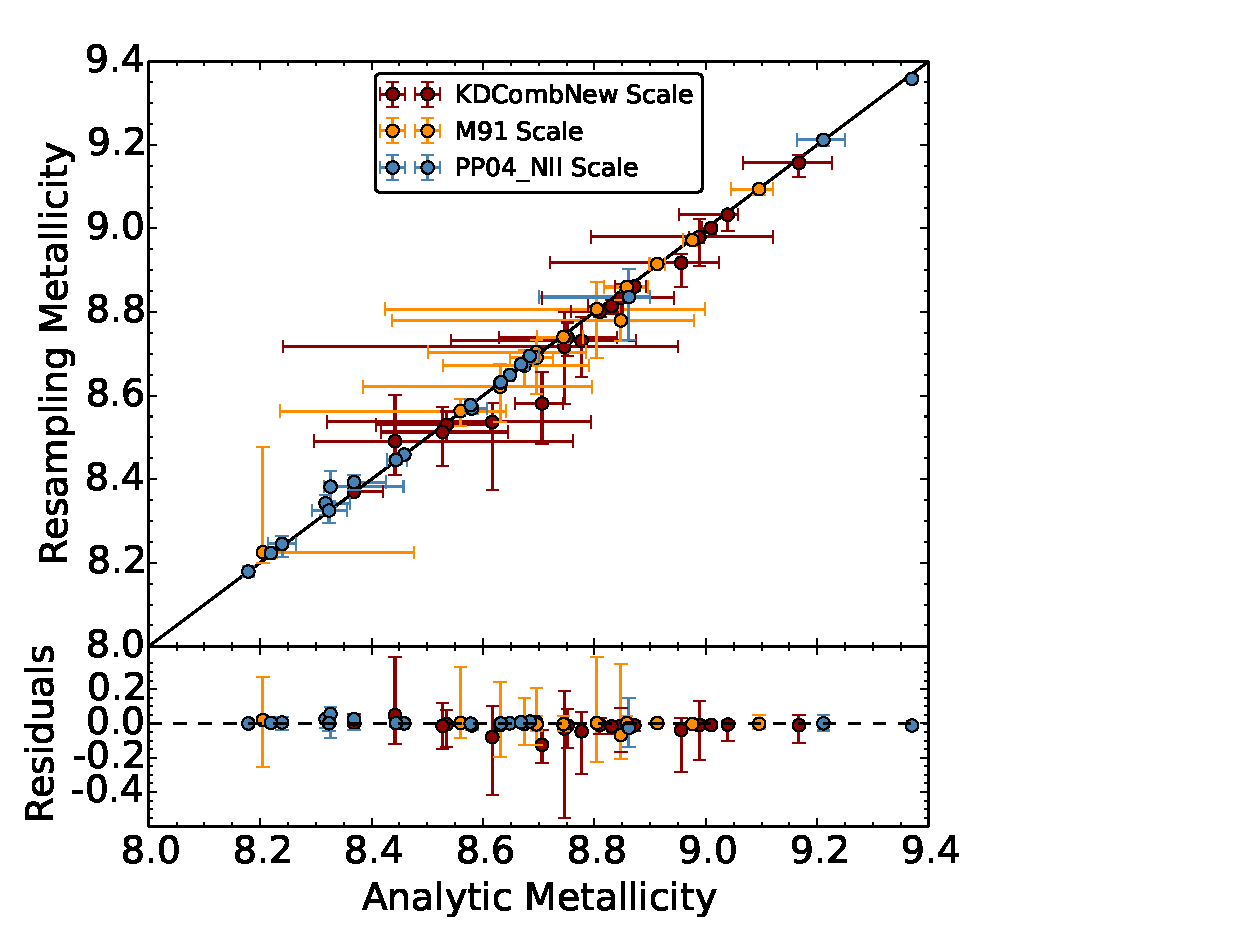
\includegraphics[trim = 10mm 0mm 10mm 0mm, clip]{abcomparison6.eps}
  \includegraphics[width=0.95\columnwidth]{exampledata_n2000_PP04_O3N2_1KDE.pdf}
   \caption{\textbf{FINISH}}
\label{fig:KDE}
\end{figure}
Lastly, we enable the user to obtain a distribution Kernel Density if the \verb=sklearn= is available. The Kernel Density of the distribution is then calculated via  \emph{KD Tree} with a top-hat function, as explained in the sklearn package documentation \footnote{\url{http://scikit-learn.org/stable/modules/density.html}}. The results will then show both a histogram, with $N_\mathrm{bins}$ chosen via Knuth's method, as well as the distribution Kernel Density, as shown in Figure~\ref{fig:KDE}.


\begin{figure}[ht!]
%  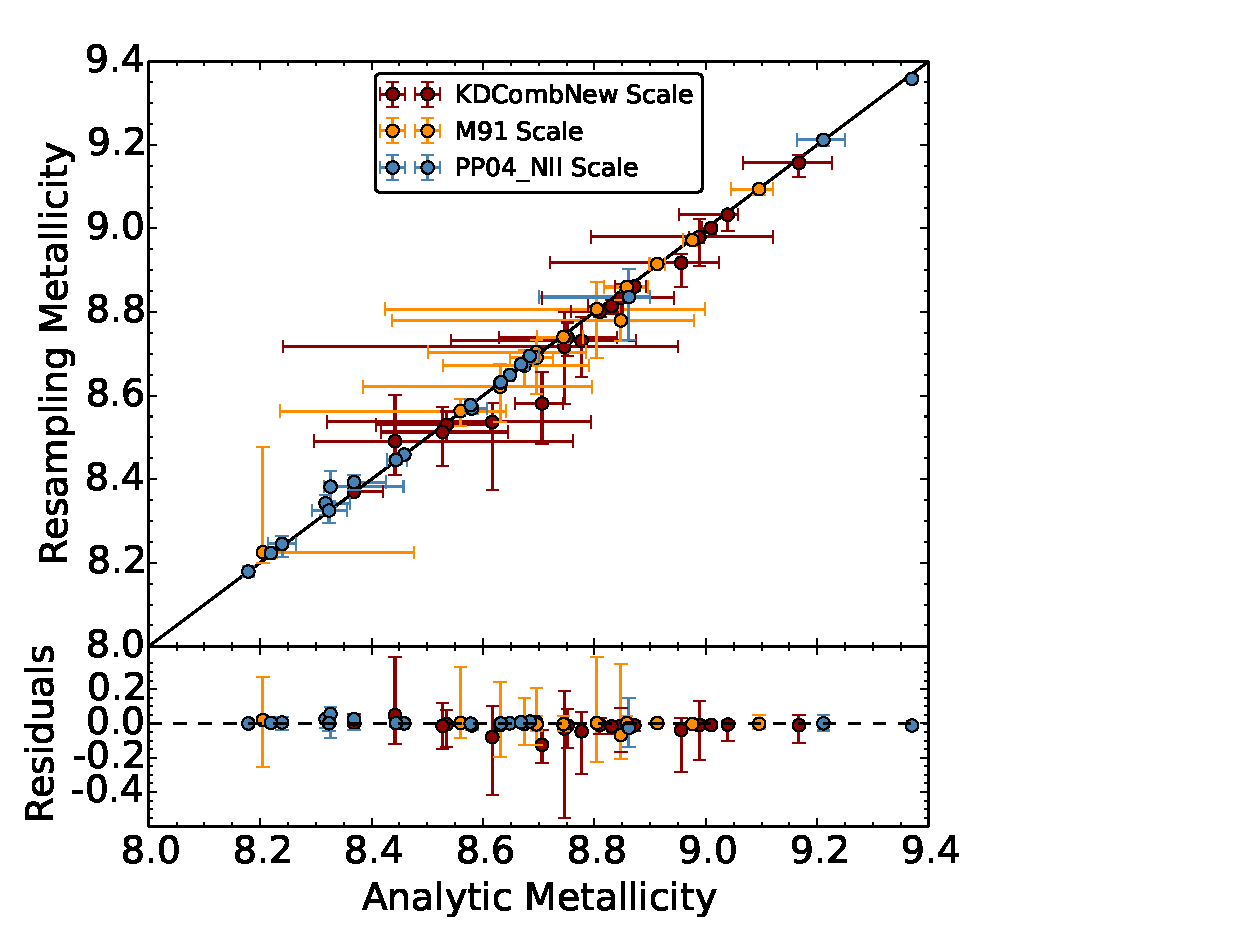
\includegraphics[trim = 10mm 0mm 10mm 0mm, clip]{abcomparison6.eps}
  \includegraphics[width=0.95\columnwidth]{exampledata_boxplot2000_m1.pdf}
   \caption{\textbf{FINISH}}
 \label{boxplot}
\end{figure}

The boxplot summarizes the resut from each scale the user chooses to calculate. For each scale a box is shown, and the box height represents the 25\% percentile of the \oxab~ distribution. Inside the box a black line represents the distribution median, the bars represent the maximum and minimum value of the distribution, excluding outliers, and the outliers are plotted as circles, and are defined as all datapoints more than one and a half times the length of the box from either end of the box (or 1.5xIQR, where IQR is the the \emph{interquartile range}). The solar oxigen aboundance is indicated in this plot for comparison: a gray box shows a range of estimated values for solar oxigen aboundances, from \oxab=8.69 \citep{Asplund09} to \oxab=8.76 \citep{Caffau11}. 
Notice that only the diagnostics requested by the user have a slot in the plot (in the example in Figure~\ref{fig:KDE} the computed scales are M91, the PP04 scales, and the KD02 scales. However these slot exists on the plot whether the diagnostic can be produced or not, i.e. if the input lines to not allow a requested scale to be calculated an empty coulmn will be generated in this plot in correspondence of said metallicity scale.\

%Using a bin size of $\sqrt{N}$ was recommended, but this proved to be slightly over-fitting, and after a number of tests, we found $2* \sqrt[3]{N}$ to be appropriate for most cases.

% While the histograms at sufficiently high $N$, where $N$ is the total number of iterations, yielded single peaked results, at lower $N$ there were occasional multiple peaks resulting from a non-smooth gaussian being sampled. In selecting the value of $N$, we found that around $N=20,000$ the KS tests showed the same distributions as larger sized samples, i.e. that the results converged ({\bf FED CHECK MY WORDING!}). 









\section{Comparison to prior uncertainty computation and other works }\label{comp_sec}


A previous method for determining the uncertainty in the oxygen abundance (as used in \citealt{modjaz08_Z,kewley10,rupke10,modjaz11}) was an \emph{analytic} approach of propagating the emission-line flux uncertainties: it found the maximum and minimum abundances via maximizing and minimizing, respectively, the various line ratios by adding/subtracting to the measured line values their uncertainties. For comparison we computed the metallicities and their errors in both ways (both analytic and using our current MC resampling method) for 3 representative scales. We plot our results and the residuals in Fig.\ref{comp_anal_MC}, which shows a number of important points: i) The metallicity reported as the 50th percentile of the metallicity parameter distribution from the MC resampling method is completely consistent with the analytically derived metallicity -  well within the respective error bars - and thus, the prior published results still stand (unsurprisingly, since our code, aside for the calculation of the confidence interval, uses the same algorithms developed for IDLKD02). ii) The MC resampling method has smaller error bars than the analytic method, especially for the scales of M91 and KD02. This is easily understandable, since the analytic method assumes the worst-case-scenario, as it basically yields 2 metallicity parameter draws (the "minimum" and "maximum") which are in the tail of the full metallicity probability distribution. However, the MC resampling method is the more appropriate method as it empirically characterizes the full parameter estimation distribution.
%assumes that \textbf{all} emission line measurement have been drawn from the 68\% tail of the error distribution and 

\begin{figure}[ht!]
%  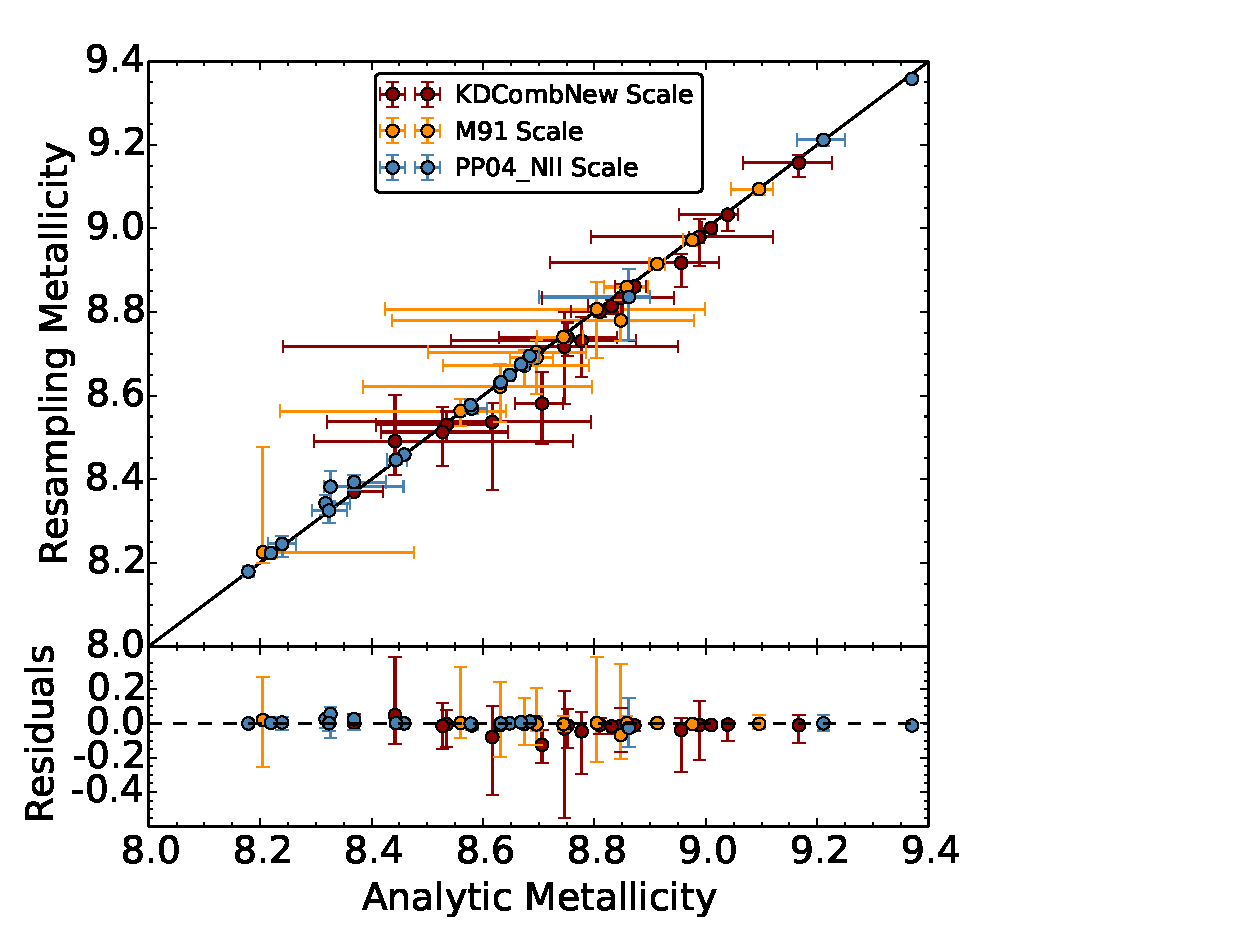
\includegraphics[trim = 10mm 0mm 10mm 0mm, clip]{abcomparison6.eps}
  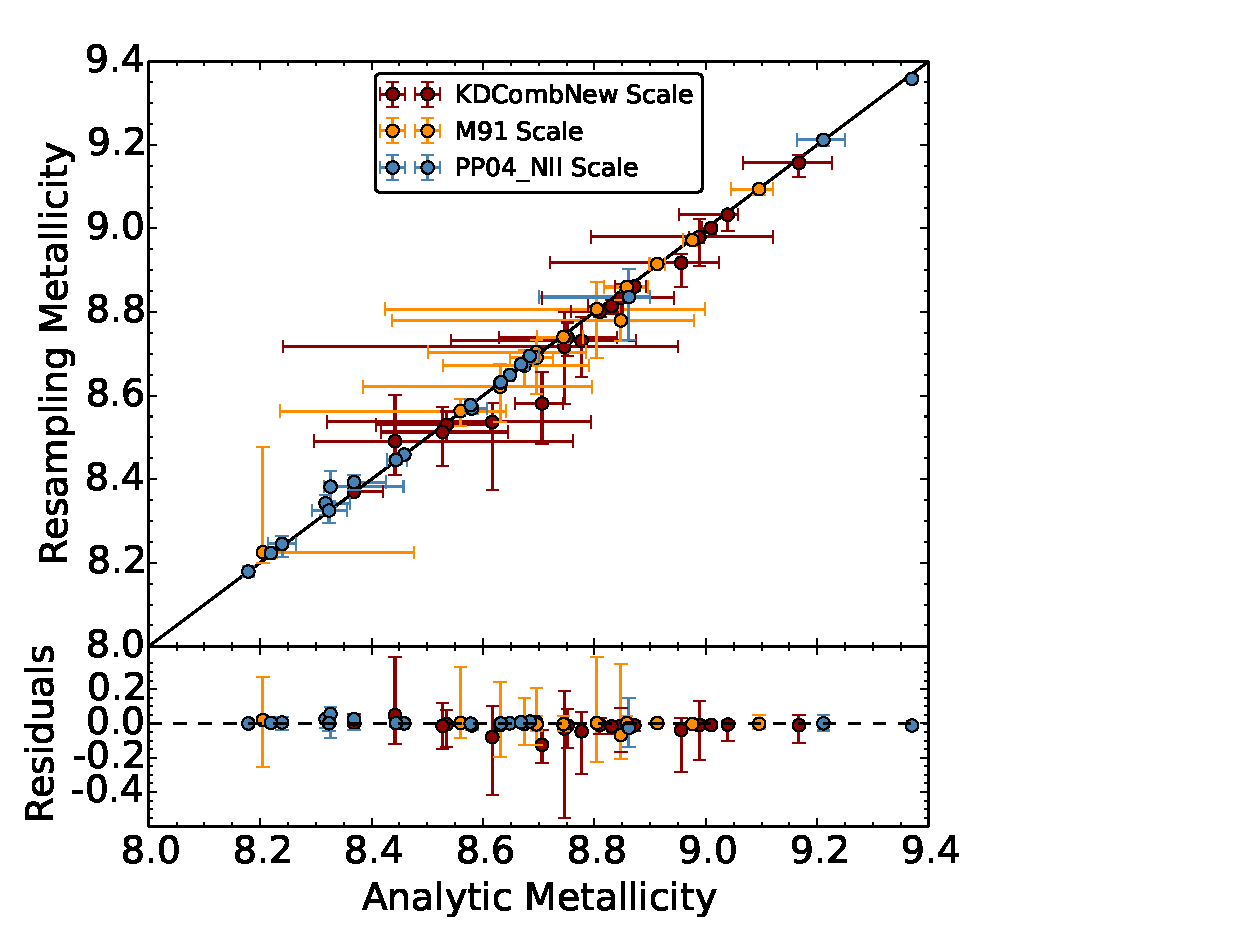
\includegraphics[width=1.2\columnwidth]{abcomparison6.eps}
   \caption{\textbf{FINISH}.Comparison of metallicity estimation between the analytic method and our Monte Carlo resampling method (top) and their residuals (bottom) for 3 different metallicity scales. Flux measurements come from 19 galaxies previously measured in \citet{modjaz11}. To add asymmetric errors in quadrature we use $residual_{min}=\sqrt {x_{max}^2 + y_{min}^2}$ and $residual_{max}=\sqrt {x_{min}^2 + y_{max}^2}$}
 \label{comp_anal_MC}
\end{figure}




%Although the flux probability distribution function is assumed to be symmetric, the metallicity errors are asymmetric because they are derived from the log of minimized and maximized flux ratios.
%Rupke: Errors were propagated primarily using analytic expressions, but for abundance and gradient errors we employed Monte Carlo methods.

\subsection{Comparison with other works}

%Here we perform a literature review of both 


The field of SN host metallicity studies has been rapidly developing as these kinds of studies may be crucial avenues for constraining the progenitor systems of different kinds of explosions - however, a few of the works do not even compute errors and others not show how they compute their statistical errors or  (e.g., \citet{anderson10,leloudas11,sanders12,leloudas14}). While \citet{sanders12} compute the line flux errors from a Markov-Chain Monte Carlo fitting of a gaussian to the emission lines, they only mention in passing that they propagate the line flux uncertainties into the metallicity measurements, but do not describe how {\bf this is a little harsh, right? i think mentioning it without explaining is generally the standard for iid errors -> Maryam: " How would you rephrase it then? " }.

%by propagation of the uncertainties in the line flux measurements
%and the 0.07 dex diagnostic systematic error.
%( line flux errors from MCMC fitting of a gaussian to emission lines)

In contrast, the general metallicity field has considered in detail how to estimate the uncertainties in measured metallicities- however, none of those codes are open-source and many of them are for specific scales which were chosen by the authors:  \citet{moustakas10} also use MC resampling to estimate the metallicity uncertainties (in their case using 500 trials which seems to lead to a Gaussian distribution) but only do this for two scale, KK04 and \citet{pilyugin05}. For computing the metallicities of the SDSS star forming galaxies, \citet{tremonti04} fit a combination of stellar population synthesis and CLOUDY ({\bf citation}) photoionization models to the observed strong emission lines [OII], $H\beta$, [OIII], $H\alpha$, NII and SII and report the median of the metallicity likelihood distribution as the metallicity estimate, with the width of the distribution giving the 1 $\sigma$ (Gaussian) error. However, this is constitutes their own scale (the T04 scale).

In the last stages of preparing this manuscript \citet{blanc15} was published.  \citet{blanc15} employ Bayesian inference for doing something similar to \citet{tremonti04} - they use Bayesian inference to derive the joint and marginalized posterior probability density functions for metallicity $Z$ and ionization parameter $q$ given a set of observed line fluxes and an input photoionization model. They provide a publicly available IDL implementation of their method named $IZI$ (inferring metallicities (Z) and ionization parameters) on the author's website.


\section{Conclusions}\label{comp_sec}

 \textbf{FINISH}. We hope that this open-access code will be used in many different fields where gas-phase metallicities are important, including in the emerging field of SN and GRB host galaxies, where either it is not described how they got  or no error bars are computed (e.g., \citealt{lunnan14}). GIven its public-access nature, the users are free to include any new metallicity diagnostics, e.g., that suggested by \citet{dopita13}.

\acknowledgements
M. Modjaz is supported in parts by the NSF CAREER award AST-1352405 and by NSF award AST-1413260. FBB is supported by a \emph{James Arthur Fellowship} at the NYU-Center for Cosmology and Particle Physics. Some plots are  produced with public code DOI:10.5281/zenodo.15419 available at \url{https://github.com/fedhere/residuals_pylab}.
 This research made use of NASA Astrophysics Data
System; the NASA/IPAC Extragalactic Database (NED), which
is operated by the Jet Propulsion Laboratory, California Institute
of Technology, under contract with the National Aeronautics
and Space Administration.



%\epsscale{1.0}
%\begin{center}
%\csvautotabular{table1.csv}
%\label{t1}
%\caption{Comparison of M-M method with MC method}
%\end{center}
%\end{figure*}



%%%%%%%%%%%%%%%%%%%%%%%%%%%%%%%%%%%%%%%%%%%
%%\clearpage
%%%%%%%%%%%%%%%% BIBLIOGRAPHY  %%%%%%%%%%%%%%%%%%%%%%%% 
\bibliographystyle{apj}
%\bibliography{refs}
\bibliography{refs}

\appendix

\section{Minimum Code validation}
\textbf{WORK WITH FED - and any other code specific things}
\end{document}


@INPROCEEDINGS{astroML,
  author={{Vanderplas}, J.T. and {Connolly}, A.J.
          and {Ivezi{\'c}}, {\v Z}. and {Gray}, A.},
  booktitle={Conference on Intelligent Data Understanding (CIDU)},
  title={Introduction to astroML: Machine learning for astrophysics},
  month={oct.},
  pages={47 -54},
  doi={10.1109/CIDU.2012.6382200},
  year={2012}
}}

@BOOK{astroMLText,
  title={Statistics, Data Mining and Machine Learning in Astronomy},
  author={{Ivezi{\'c}}, {\v Z}. and {Connolly}, A.J.
          and {Vanderplas}, J.T. and {Gray}, A.},
  publisher={Princeton University Press},
  location={Princeton, NJ},
  year={2014}
}

%,page]{appendix}
%\usepackage{amsmath}
%\usepackage{amssymb}
%\usepackage{verbatim}
%\usepackage{graphicx}
%\usepackage{epsfig}
%\usepackage{morefloats}
%\usepackage{float}
%\usepackage{lipsum}
%\usepackage{subfigure}
%\usepackage{longtable}
%\usepackage{lipsum} 
%\usepackage{rotating}
%\usepackage{wasysym}

\begin{document}
\title{Monte Carlo Method for Calculating Uncertainty in Oxygen Abundance from Strong-Line Flux Measurements}

\author{Author order to be determined: Maryam Modjaz\altaffilmark{1}, Federica B. Bianco\altaffilmark{1}, Seung Man Oh\altaffilmark{1,2}, David Fierroz\altaffilmark{1}, Yuqian Liu\altaffilmark{1}, Lisa Kewley\altaffilmark{3,4}}
\altaffiltext{1}{Center for Cosmology and Particle Physics, New York University, 4 Washington Place, New York, NY 10003, USA}
 \altaffiltext{2}{NYU Abu Dhabi PO Box 129188 Abu Dhabi, UAE}
 \altaffiltext{3}{Australian National University, Research School for Astronomy \& Astrophysics, Mount Stromlo Observatory, Cotter Road, Weston, ACT 2611, Australia }
 \altaffiltext{4}{ Institute of Astronomy, University of Hawaii, 2680 Woodlawn Drive, Honolulu, HI 96822, USA}
 
 
\begin{abstract}
\textbf{MODIFY \& FINALIZE AT THE END:} We present an open-source Python code for the determination of the strong-emission-line estimators of oxygen abundance in the standard scales, based on the original IDL-code in \citet{kewley02}. The standard strong line Metallicity scales and diagnostics \text{IMPROVE} have been used to estimate metal abundance through emission line ratios. Here we introduce a Monte Carlo resampling of these methods in order to better characterize an oxygen abundance confidence region.  We output median values, 16th and 84th percentile confidence regions, for various standard metallicity diagnostics, and, when possible, for reddening E(B-V). We produce Monte Carlo parameter distributions for the oxygen abundance and when possible for reddening E(B-V). We test our code on emission lines measurements from a sample of galaxies ($z<0.15$) and compare our metallicity results with those from previous methods. We show that our metallicity estimates are consistent with previous methods but yields smaller uncertainties. The code is open source and can be found at www.github.com/nyusngroup/ \textbf{
(add repo and DOI)}.
\end{abstract}
 
\section{Introduction}
The low quantity of carbon, oxygen, nitrogen, sulfur and iron among other elements provide a splash of color to the otherwise dominating greyscape of hydrogen and helium in the stars and gas of galaxies. Nevertheless, even the minute presence of heavy elements (all elements heavier than H and He, also called metals or collectively metallicity) is important for many areas of astrophysics. For example, \citet{johnson12} suggest that if it was not for the relatively high metallicity level in our Solar System, planet formation may not have been possible. With $Z$ representing the mass fraction of metals, for our own Sun the value is measured to be  Z=0.0153 \citep{chaffau11}, though there are others who suggest a lower solar metallicity of $Z=0.0134$ in particular because of oxygen \citep{asplund09_rev,grevesse10}\footnote{Note that these abundances refer to the current abundances in the sun, which are lower than the value with which the sun was formed 4.56 Gyr ago, since diffusion at the bottom of the convection zone has decreased metallicity over time \citep{grevesse10}.}. Furthermore, when properly observed and estimated, metallicity measurements of galaxies can tightly constrain models of galaxy formation and evolution (e.g., \citealt{kewley08} and references therein), tas well as shed light on the metallicity dependence and production conditions for different types of SNe and long-duration GRBs (e.g., \citealt{modjaz08_Z,levesque10_grbhosts,anderson10,modjaz11,kelly12,sanders12,lunnan14,leloudas14}), to just name a few examples.

%chaffau Z=0.0209 12+log=O/H) = 8.76�0.07 i
%Small variations in chemical abundance can often be critical indicators for stellar and galactic properties like age and activity.
%Metals are produced in the cores of stars during their fusion lifecycle but also during the extreme conditions of stellar explosions. For example, the majority of iron comes from thermonuclear explosions (SN Ia) while nearly all of oxygen is the result of core collapse (SN Ib, Ic, \& II). Since new stars are born from the clouds these explosions produce, metallicity will increase with each passing generation. Stars like our Sun, which are results of multiple generations of star formation, are often found in the more active parts of the galaxy, such as the disk, and are referred to as Population I stars. Population I stars have higher metallicity than older Population II stars, which are also present in the disk but are the exclusive members of the low activity galactic halo. Population III stars would be first generation stars with zero metallicity, but have yet to be observed.
%Besides age, metallicity also influences stellar temperature. Metals are more effective at absorbing energy coming from the interior of the star in the stellar atmosphere so their presence increases the stellar opacity. With greater absorption and opacity the radius expands to a size larger than it would be without metals and this larger size results in a cooler effective temperature. While metallicity can help indicate age or activity it's temperature and density dependencies require parameterization to properly be estimated.

However, for almost all astronomical objects, metallicity cannot be measured directly. The oxygen abundance in the gas-phase is the canonical choice of metallicity indicator for interstellar medium (ISM) studies, since oxygen is the most abundant metal and only weakly depleted onto dust grains (in contrast to refractory elements such as Mg, Si, Fe, with Fe being depleted by more than a factor of 10 in Orion; see \citealt{simondiaz11-orion}). The oxygen abundance\footnote{We note that in many cases in the literature, including here, the terms metallicity and oxygen abundance are used interchangeably.} is expressed as  $12 + \log_{10}(\frac{O}{H})$, where $O$ and $H$ represent the number of Oxygen and Hydrogen atoms, respectively. Importantly, oxygen exhibits very strong nebular lines in the optical wavelength range of HII regions (e.g., \citealt{pagel79,osterbrock89,tremonti04}), and thus, many different diagnostic techniques, relying on different lines, have been developed (e.g., \citealt{kewley02,pettini04,kobulnicky04,kewley08}), which are discussed in the next section.

\subsection{The different oxygen abundance diagnostics}
Here we present a brief overview of the various observational methods for measuring the gas-phase oxygen abundance - however, for a full discussion with all the caveats we encourage the reader to see reviews by e.g. \citet{stasinska02,kewley08,moustakas10,stasinska10,dopita13,blanc15}.
The so-called ``classical'' way to estimate the oxygen abundance is the electron temperature ($T_e$) method, which estimates the electron temperature and density of the nebula using a number of oxygen lines with different ionization states, including the auroral [OIII] $\lambda$4363 line, to then directly estimate the OII and OIII abundances to obtain the total oxygen abundance, after correcting for the unseen stages of ionization. However, the auroral [OIII] $\lambda$4363 line is very weak, even in low-metallicity environments, and saturates at higher metallicity (since at higher metallicities the cooling is dominated by the Oxygen NIR fine structure lines) $-$ thus, other methods had to be developed that use other, stronger lines, in the spectra of HII regions. These are called strong-line methods and are the subject of this manuscript. Strong-line methods can be categorized into two types: theoretical methods, that rely on calibrating various observed line ratios using photoionization methods (basically theoretically simulating HII regions, using stellar model atmospheres, stellar population synthesis and photoionization models) and empirical ones that calibrate various observed strong line ratios using observed $T_e$-based metallicities. While historically there have been large systematic offsets between the $T_e$ method and the strong line methods, \citet{dopita13} demonstrated that the $T_e$ method gives the same results as the strong line methods, if the energy distribution of the electrons in the HII regions is assumed to not be a simple Maxwell-Boltzmann distribution (as assumed in prior works), but a more realistic $\kappa$ distribution, as observed in solar system astrophysical plasma. They also find that the effect of the $\kappa$ distribution on the strong-line methods is minor.


For the theoretical strong-line method, one ratio that is commonly used to determine the metallicity of galaxies is ([OII] $\lambda 3727$ $+$ [OIII] $\lambda 4959,\lambda 5007$)$/$H$_\beta$ \citep{pagel79} and is referred to as R23. The drawback of this method is that it is double-valued with metallicity, and thus other line ratios need to be used to break the degeneracy between the high values ("upper branch") and the low values ("lower branch") of the R23 metallicities. Furthermore, \citet{kewley02} showed the importance of ionization parameter, which can be physically understood to correspond to the maximum velocity of an ionized front that can be driven by the local radiation field of hot massive stars that are ionizing the ISM gas. This ionization parameter needs to be taken into account in the various strong-line methods, as HII regions at the same metallicity but with different ionization parameters produce different line strengths. Calibrations of R23 by \citet{mcgaugh91} (hereafter M91) and by \citet{kewley02} (hereafter KD02) use different theoretical photoionization models and take the ionization parameter into account, while other calibrations such as of \citet{zaritsky94} (hereafter Z94) do not. Thus, Z94 is mostly valid for only metal-rich galaxies.  M91 and KD02 use an iterative process to break the R23 degeneracy  (KD02 uses different ratios [NII]$/$[OII] and [NII]$/$H$_\alpha$) and to also constrain the ionization parameter $q$ in order to arrive at the metallicity estimate.

%The most direct way to estimate metallicity in spectra is to measure line fluxes absorbed or emitted by metals and non-metals. While iron lines may be present in stellar spectra, iron is less commonly found in gaseous nebulae than oxygen is. Not only is oxygen more abundant but it emits several strong lines ([OI] $\lambda 6300$, [OII] $\lambda 3727,7318,7324$, [OIII] $\lambda 4363, 4959, 5007$) visible at optical wavelengths that can also be used to quantify temperature and density. For this reason 
%While the ratio of oxygen to hydrogen line flux correlate with metallicity, the ratio of two [OIII] lines, one auroral $\lambda 4363$ and the other an excitation line at $\lambda 5007$ can be used to determine what is called the Ionization Correction Factor (ICF) (Kewley \& Dopita 2002).
As to empirical strong-line methods, the most commonly used one is that by \citet{pettini04} (hereafter PP04). PP04 used HII regions with $T_e$-based metallicities to derive empirical fits to strong-line ratios, and introduce the line ratios of ([NII]$/$H$_\alpha$ (N2) and ([OIII]$/$H$_\beta$)$/$([NII]$/$H$_\alpha$ (O2N2) as metallicity diagnostics. Since PP04-N2 employs two closely spaced lines (Halpha and NII), which are not affected by stellar absorption, nor uncertain reddening, and are easily observed in one simple spectroscopic setup, it has become an often-used scale for at least low-z SN host galaxy studies (e.g. see metal-analysis by e.g,. \citealt{sanders12,modjaz12_proc,leloudas14}). However, it is important to remember that this scale has a number of short-comings: it does not take into account the impact of the ionization parameter, it was initially derived based on only 137 extragalactic HII regions, and the nitrogen emission line employed saturates at high metallicity (\textbf{CHECK!}), and thus this method may not be well-suited for high-metallicity galaxies. An updated calibration by \citet{marino13} based on many more Te-based metallicities (almost three time larger that that of PP04) derives a significantly shallower slope between O3N2 index and oxygen abundance than the PP04 calibration.


As it can be seen, each scale has different advantages and disadvantages and should be used in different metallicity regimes (see detailed discussion in e.g.,  \citealt{kewley02,stasinska02,kewley08,moustakas10,dopita13,blanc15}). Thus, this open-source code outputs the oxygen abundance in the main 6 metallicity scales (for which the KD02 diagnostic has four outputs and the PP04 diagnostic has two outputs). While there is a long-standing debate about which diagnostic to use, as there are systematic metallicity offsets between different methods (recombination lines vs.  strong-line method vs. ``direct'' $T_e$ method, see the above sources), \emph{\bf the relative metallicity trends can be considered robust, if the analysis is performed self-consistently in the same scale, and trends are seen across different scales \citep{kewley08,moustakas10}}. Note however, that while there are conversion values between different scales \citep{kewley08}, they apply for large data sets, since those conversion values were derived based on ten thousands of SDSS galaxies, and thus should be used with caution (or not at all) for smaller samples. In addition, one should note that there is a debate about the value of the solar oxygen abundance \citep{asplund09_rev,chaffau11}, such that the absolute oxygen calibration is still uncertain.




Here we introduce the open-source python code "". pro .. In \S~\ref{method_sec} we describe our method, the input and output values of the code. In \S~\ref{comp_sec}, we compare our method of obtaining abundance uncertainties to previous methods in the literature. 
%\begin{figure}[H]
%\epsscale{1.0} 
%\begin{center}
%\includegraphics[width=0.89\columnwidth]{fig1.png} 
%\caption{Example of a sampled Gaussian. 50,000 points from a Gaussian distribution were selected in this case}
%\label{f1}
%\end{center}
%\end{figure}


\section{Description of Metallicity code}\label{method_sec}


\begin{figure*}[!HT]
%\epsscale{0.6}
\begin{center}
\centerline{
\includegraphics[width=0.95\columnwidth]{exampledata_n2000_KD02comb_1.pdf}
%exampledata_n50000_KD02comb_updated_1.ps}
\includegraphics[width=0.95\columnwidth]{exampledata_n2000_PP04_O3N2_1.pdf}}
%exampledata_n50000_PP04_O3N2_1.ps}
\vspace{0.2in}
\centerline{
\includegraphics[width=0.95\columnwidth]{exampledata_n2000_M91_1.pdf}
% exampledata_n50000_M91_1.ps}
\includegraphics[width=0.95\columnwidth]{exampledata_n20000_E(B-V)_1.pdf}}
%exampledata_n50000_EBV_1.ps}

\caption{WILL UPDATE WITH NEW FIGURES BASED ON A PUBLISHED SN WITH SIGNFICANT E(B-V) AND WRITE MORE TEXT. Metallicity and reddening ($E(B-V)$) parameter distributions based on example data (namely, emission line data of the HII regions at the position of SN~2008D, published in \citet{modjaz11}, based on $N$=20,0000 samples. The median value is shown with the dashed lines, while the 16th till 84th confidence region is shaded in tan color. The shown metallicity scales are  by \citet{kewley02}, updated by \citet{kewley08} (KD02combupdated), \citet{pettini04}, using OIII and NII  (PP04-O3N2) and \citet{mcgaugh91} (M91). These are the same plots that are outputted by the code, which produces such plots for all scales (namely those of s\textbf{LIST THEM ALL}). The legend also includes the ID number of }
 \label{metallicity_distribution}
\end{center}
\vspace{-0.5in}
\end{figure*}


For computing oxygen abundances, we use the iterative code by \citet{kewley02}, which has been updated in \citet{kewley08} and reflects .. \textbf{LISA: YOUR INPUT HERE:what is the update??} which was initially written in IDL.  We translated the code into python, added the new feature of obtaining uncertainties on the metallicity outputs via Monte Carlo resampling, and made it open source via github, as we explain below.

We assume that the observed emission lines to be used to indicate metallicity originate in HII regions and are not due to non-thermal excitation by e.g., AGN or interstellar shocks from SNe or stellar winds.  Tests to exclude data contaminated by such non-thermal sources should be executed using the recommended line ratios by e.g., \citealt{baldwin81,kauffmann03,kewley06_sdss} prior to running this code. Furthermore these lines should have all the correct calibration (at least correct relative calibration) and should have a signal-to-noise ratio (S/N) of at least 3. The latter is important for the success of the Monte Carlo resampling technique as described below.

\subsection{Input and Output of code}
Emission line flux values are fed into our Python implementation as in the original IDL code by \citet{kewley02}, hereafter referred to as IDLKD02. The inputs are emission line flux values and their uncertainties for the following lines: H$\alpha$, H$\beta$, [OI] 6300, [OII] 3727, [OIII] 4959, [OIII] 5007, [NII] 6584, [SII] 6717, [SII] 6731, SIII 9532, and SIII 9096 \textbf{CHECK AT THE END WITH CODE!} and their uncertainties (consult the README.md in the github repository for details about the input format). If the fluxes for the specified lines are not available, the entry is left to 0 \textbf{FED: we should do NaN!???} and the outputted oxygen abundance scales will be in only metallicity scales that use the provided line fluxes. As part of the code, the inputted line fluxes are corrected for reddening by using the observed Balmer decrement, for which H$\alpha$ and  H$\beta$ flux values need to be provided. We assume case B recombination, and thus the standard value of 2.86 as the
intrinsic H$\alpha$/H$\beta$ ratio \citep{osterbrock89}, and apply the standard Galactic reddening law with $R_V$ = 3.1 \citep{cardelli89}. However, the user can choose other extinction laws and $R_V$ values, if desired, given the code's open-source nature.

While other parameters, such as the ionization parameter $q$ and the electron density (using the SiII lines) are computed as long as the necessary lines are provided, they are not outputted in the current version of our code $-$ however, the reader is welcome to easily modify the code to suite their needs, given it's an open-source code.

As output, we obtain metallicity values and their uncertainties in the following calibrations, as discussed in detail in \citet{kewley02,kewley08}: \citet{kewley02}(KD02, for the 4 following computations: R23, using the NIIOII ratio, using the NII/Halpha ratio, and a combined method that uses the optimal method given the input line fluxes), \citet{mcgaugh91} (M91), \citet{zaritsky94} (Z94), \citet{pilyugin01} (P01), \citet{denicolo02} (D02), 
\citet{pettini04} (2 computations: PP04-N2, PP04-O3N2) \textbf{CHECK WITH FINAL CODE - ALSO CHECK whether P01 is P01 or P05 by looking at the code}. If the line fluxes necessary for specific scales are not provided, the output  metallicities will default to -1, if the errors in he measurements are not provided, the code will specify that it cannot create a measurement distribution and determine a confidence interval.



\subsection{Computing Uncertainties}
The novel aspect of our work is that for every set of input line measurements we introduce a Monte Carlo (MC) resampling method to obtain iterations via random sampling within the measurement errors, and thus we obtain a robust result for error estimation (e.g., \citealt{efron79,hastie09,andrae10}). 

Given a data set with error bars from which certain parameters are estimated, Monte Carlo resampling generates synthetic data samples drawing from a given distribution. 
Here we draw synthetic data from a Gaussian distribution centered on each measured line flux value, with standard deviation corresponding to the measurement error. The implicit assumption is made, of course, that the line flux error is Gaussian distributed in nature\footnote{The user may wish to provides their own probability distribution for the emission line uncertainties, and easily modify the code to suite their needs.}. 

% FED: because we vectorize, we actually do not do this sample by sample so we cannot say ``Every iteration''
For each metallicity scale, for each of $N$  values chosen randomely within the relevant emission line distributions we run the calculations that derives the metallicity.
This effectively simulates conducting multiple experiments when repeating observations is impractical or impossible, as in the case of the emission line flux data, and thus generates alternative data sets. 
%FED redundant: We generated $N$ Monte Carlo flux samples for each emission line, and calculated the metallicity for each set of line fluxes. 
The sample size $N$ is set by the user, and one should expect an appropriate value of $N$ to be a few 1000s, depending on the metallicity scale chosen and measurement errors (for example  $N=2,000$ is determined to be sufficient for our example data, as shown below, and we provide tools to assure the sample size is sufficiently large). 
%FED: note that 2000 is ok for our sample but it does not need to be! it depends on the error size, and the shape of the distribution, so it depends on the input. if for example the distribution 
% , FED: because we vectorize, we actually do not do this sample by sample, so we cannot say ``At the end of $N$ iterations''
A parameter estimate distribution of oxygen abundance is generated for each scale, the metallicity and its confidence region are calculated,
%We bin to visualize, but we calculate percentiles on the actual distribution
and the results are bunned abd visualized in a histogram (see below)\footnote{However, note this method is a conservative approach, since it overestimates the intrinsic metallicity uncertainty, as we are centering this error distribution on the measured values instead of the (unknown) true values \citep{andrae10}.
%FED i do not know what that means. i would think that this method is NOT conservative on account of that!
}. This is done for each scale the user chooses to calculate. The fiftieth (50\%) percentile, i.e.  the median, is reported as the measuredtrue metallicity value, and the 16th and 84th percentiles of the distribution as its confidence region. %FED redundant? The output of our code includes the oxygen abundance measurements plus confidence regions in all scales, as well as plots of the distributions of the oxygen abundance value in all scales. 

This MC resampling approach takes into account the impact of the uncertain reddening (due to the uncertainties in the measurement of the 
H$\alpha$ and H$\beta$ fluxes), when the option for de-reddened metallicities is chosen. Since for each iteration, a new reddening value is calculated based on the resampled H$\alpha$ and H$\beta$ fluxes, which is used to compute the de-reddened metallicity value, the derived distribution of metallicity values takes into account the uncertain redding. As part of the output, a probability distribution plot for E(B-V) is provided (see last plot in figure~\ref{metallicity_distribution}, along with confidence intervals derived using the same method as for the metallicity measurements. If either H$\alpha$ or H$\beta$ flux is not provided, then no reddening correction can be applied and the computed metallicity will not be  reddening-corrected and the E(B-V) output will be set to zero.

Figure \ref{metallicity_distribution} shows the metallicity estimate distribution for 3 representative scales, and for the reddening parameter E(B-V) - similar plots that are outputted by our code for all scales as listed above (not all shown here). Although the input distributions are Gaussian, the metallicity distributions 
%FED: in log space they are NEVER gonna be gaussian so not ``rarely are'',
are not, for two reasons: first, since the metallicities are computed based on log values of line flux ratios, symmetric error bars in linear space will translate into asymmetric error bars in log space; and second, some metallicity computations are non-linear, and (especially those that include $R_{23}$) sometimes bimodal since they choose upper vs lower branch to break degeneracy.

Since the metallicity distributions are rarely Gaussian, the percentiles we report cannot be expressed in terms of $\sigma$ values. In determining the confidence region intervals for asymmetric and multi-modal distributions, there are broadly three approaches (e.g., \citealt{andrae10}): choosing a symmetric interval, the shortest interval,  or a ``central'' interval.  With the "central" method we determined the  confidence interval by choosing the left and right boundaries such that the region outside the confidence interval each equally contains $16\%$ of the total distribution - in analogy to the one-sigma-interval of the Gaussian distribution. This ensures that the algorithm finds the proper boundaries even for asymmetric, non-Gaussian, distributions, (i.e., multimodal likelihood distributions) and in the case of multiple peaks. 

In summary, the output for the measured value corresponds to the fiftieth (50\%) percentile, while the lower error bar corresponds to the 50$^{th}$-16$^{th}$ percentile and the upper error bar corresponds to 84$^{th}$-50$^{th}$ of the metallicity parameter estimate distribution. However, we urge that the reader always inspect the appropriate metallicity distribution plots, which are also outputted, to check for themselves whether the outputted median and confidence regions properly represent the full metallicity distribution (see Section~\ref{visz}).

We note that our code  does not output the \emph{systematic} uncertainty of each scale, which are e.g., $\sim$ 0.07 dex (or 0.14 dex \textbf{CHECK}) for PP04-O2N2.  Thus systematic errors can be as large, if not larger, than the statistical errors, however, if all metallicity measurements are in the \emph{same} scale and only \emph{relative} comparisons are made, then the systematic error does not have any impact (by definition!). The distributions for the D02 scale include the uncertainty in the fit parameters: the oxygen aboundance in this scale is generated as \oxab~=~$9.12~\pm 0.05 + (0.73~\pm 0.10)~\mathrm{NII}$, as published in  \citet{denicolo02}. The parameter fit are generated as the sum of the nominal parameter (9.12 and 0.73) and a Gaussianly distributed random value centered on zero, and within a standard deviation of 0.05 and 0.10, respectively.

%However, the
%relative metallicity difference measured between a given pair
%of galaxies in different diagnostics is consistent with an rms
%scatter typically ?0.07 dex, and 0.15 dex between the most
%discrepant diagnostics (Kewley&Ellison 2008).


%from Kewley & Ellison08: The cause of the metallicity calibration discrepancies remains unclear. The discrepancy has been attributed to either an unknown problem with the photoionization models (Kennicutt et al. 2003) or temperature gradients or fluctuations that may cause metallicities based on the electron temperature method to underestimate the true metallicities (Stasin�ska 2002, 2005; Bresolin 2006). Until this discrepancy is resolved, the absolute metallicity scale is uncertain.

\subsubsection{Visual diagnostics}\label{visz}
In order for the user to check the validity of a measurement, and to better understand the distribution, we provide two visualizations: for each metallicity scale calculated, for each input set, we generate a histogram of the output distribution (Figure \ref{metallicity_distribution} and \ref{fig:KDE}), and for each set of input line we generate a \emph{box-and-whiskers} plot (herehance \emph{boxplot}, for short) summarizing the result of all scales calculated (Figure \ref{boxplot}). 

Choosing the binning size for a histogram is not a trivial task.  \citet{hogg08} describes various data analysis recipes for selecting a histogram bin size. Too many bins will result in many empty bins and an ``over-fit'' histogram, while too few bins may miss features of the distribution. 
By default, we use \emph{Knuth's Method} to choose the number of bins $N_\mathrm{bins}$ for each histogram. Knuth's method  optimizes  a Bayesian fitness function across fixed-width bins \citep{Knuth06}. Additionally, however, we enable a number of binning options from which the user can choose, including: 
the square root of the number of bins, \emph{Rice rule} ($N_\mathrm{bins}~=~2\sqrt[3]{N}$, e.g., \citealt{hastie09}), 
\emph{Doane's formula} ($N_\mathrm{bins}~=~1 + \mathrm{log}_2{N} + \mathrm{log}_2\left(1 + \mathrm{Kurt}\sqrt{(N / 6)}\right)$, where Kurt is the third standardized moment of the distribution \citealt{Doane76}\footnote{\citet{Doane76} attempted to address the issue of finding the proper number of bins for the histogram of a skewed distribution. Several version of the so-called Doane's formula can be found in the literature. Our formula can, for example, be found in \citealt{Pharmacokinetic}}), and the full Bayesian solution, known as Bayesian Blocks, which optimizes a fitness function across an arbitrary configuration of bins, such that the bins are of variable size \citep{scargle13}. The implementation of the latter method requires the \verb=astroML= python package to be installed on the user's system (\citealt{astroml}\footnote{\url{https://github.com/astroML/astroML}}). If the \verb=astroML= package is not found, the code will default to Knuth's Rule. 

As mentioned, Knuth's method implies an optimization. In cases in which the convergence of this minimization takes too long (or if the number of bins after the minimization is  $N_\mathrm{bins}/\sqrt{N} > 5$ or $N_\mathrm{bins}/\sqrt{N} < 1/3$) the code will revert to Rice rule.

\begin{figure}[ht!]
%  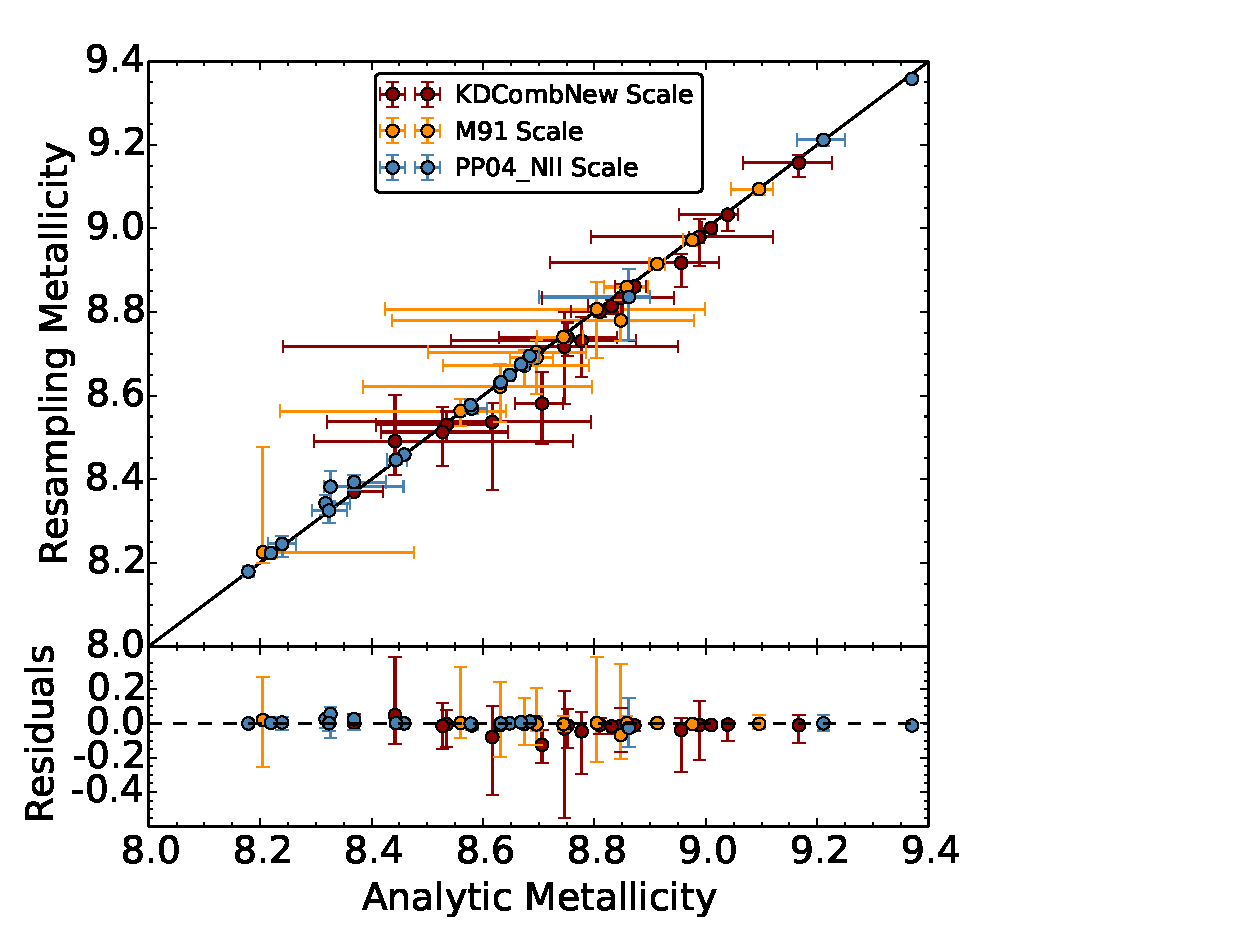
\includegraphics[trim = 10mm 0mm 10mm 0mm, clip]{abcomparison6.eps}
  \includegraphics[width=0.95\columnwidth]{exampledata_n2000_PP04_O3N2_1KDE.pdf}
   \caption{\textbf{FINISH}}
\label{fig:KDE}
\end{figure}
Lastly, we enable the user to obtain a distribution Kernel Density if the \verb=sklearn= is available. The Kernel Density of the distribution is then calculated via  \emph{KD Tree} with a top-hat function, as explained in the sklearn package documentation \footnote{\url{http://scikit-learn.org/stable/modules/density.html}}. The results will then show both a histogram, with $N_\mathrm{bins}$ chosen via Knuth's method, as well as the distribution Kernel Density, as shown in Figure~\ref{fig:KDE}.


\begin{figure}[ht!]
%  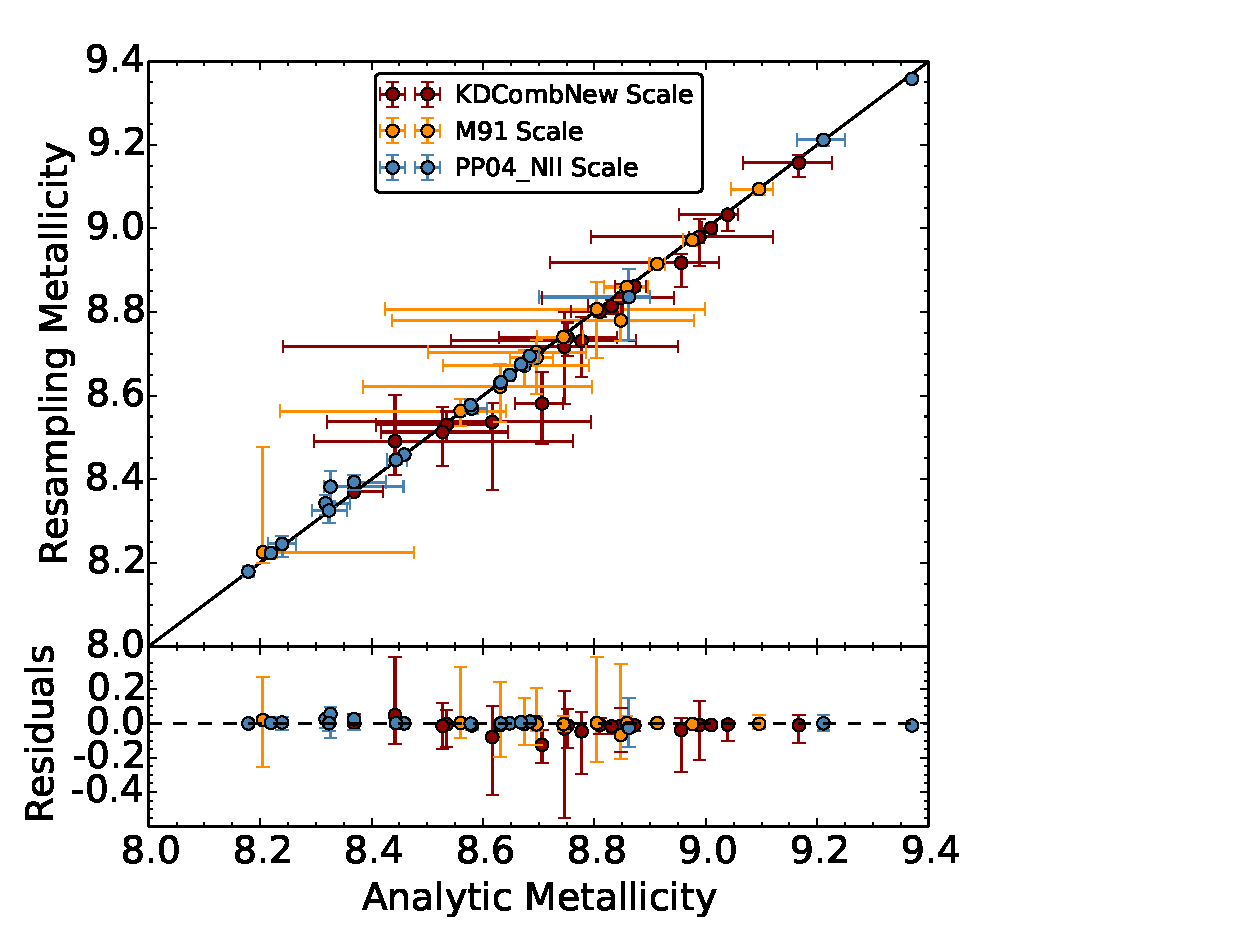
\includegraphics[trim = 10mm 0mm 10mm 0mm, clip]{abcomparison6.eps}
  \includegraphics[width=0.95\columnwidth]{exampledata_boxplot2000_m1.pdf}
   \caption{\textbf{FINISH}}
 \label{boxplot}
\end{figure}

The boxplot summarizes the resut from each scale the user chooses to calculate. For each scale a box is shown, and the box height represents the 25\% percentile of the \oxab~ distribution. Inside the box a black line represents the distribution median, the bars represent the maximum and minimum value of the distribution, excluding outliers, and the outliers are plotted as circles, and are defined as all datapoints more than one and a half times the length of the box from either end of the box (or 1.5xIQR, where IQR is the the \emph{interquartile range}). The solar oxigen aboundance is indicated in this plot for comparison: a gray box shows a range of estimated values for solar oxigen aboundances, from \oxab=8.69 \citep{Asplund09} to \oxab=8.76 \citep{Caffau11}. 
Notice that only the diagnostics requested by the user have a slot in the plot (in the example in Figure~\ref{fig:KDE} the computed scales are M91, the PP04 scales, and the KD02 scales. However these slot exists on the plot whether the diagnostic can be produced or not, i.e. if the input lines to not allow a requested scale to be calculated an empty coulmn will be generated in this plot in correspondence of said metallicity scale.\

%Using a bin size of $\sqrt{N}$ was recommended, but this proved to be slightly over-fitting, and after a number of tests, we found $2* \sqrt[3]{N}$ to be appropriate for most cases.

% While the histograms at sufficiently high $N$, where $N$ is the total number of iterations, yielded single peaked results, at lower $N$ there were occasional multiple peaks resulting from a non-smooth gaussian being sampled. In selecting the value of $N$, we found that around $N=20,000$ the KS tests showed the same distributions as larger sized samples, i.e. that the results converged ({\bf FED CHECK MY WORDING!}). 









\section{Comparison to prior uncertainty computation and other works }\label{comp_sec}


A previous method for determining the uncertainty in the oxygen abundance (as used in \citealt{modjaz08_Z,kewley10,rupke10,modjaz11}) was an \emph{analytic} approach of propagating the emission-line flux uncertainties: it found the maximum and minimum abundances via maximizing and minimizing, respectively, the various line ratios by adding/subtracting to the measured line values their uncertainties. For comparison we computed the metallicities and their errors in both ways (both analytic and using our current MC resampling method) for 3 representative scales. We plot our results and the residuals in Fig.\ref{comp_anal_MC}, which shows a number of important points: i) The metallicity reported as the 50th percentile of the metallicity parameter distribution from the MC resampling method is completely consistent with the analytically derived metallicity -  well within the respective error bars - and thus, the prior published results still stand (unsurprisingly, since our code, aside for the calculation of the confidence interval, uses the same algorithms developed for IDLKD02). ii) The MC resampling method has smaller error bars than the analytic method, especially for the scales of M91 and KD02. This is easily understandable, since the analytic method assumes the worst-case-scenario, as it basically yields 2 metallicity parameter draws (the "minimum" and "maximum") which are in the tail of the full metallicity probability distribution. However, the MC resampling method is the more appropriate method as it empirically characterizes the full parameter estimation distribution.
%assumes that \textbf{all} emission line measurement have been drawn from the 68\% tail of the error distribution and 

\begin{figure}[ht!]
%  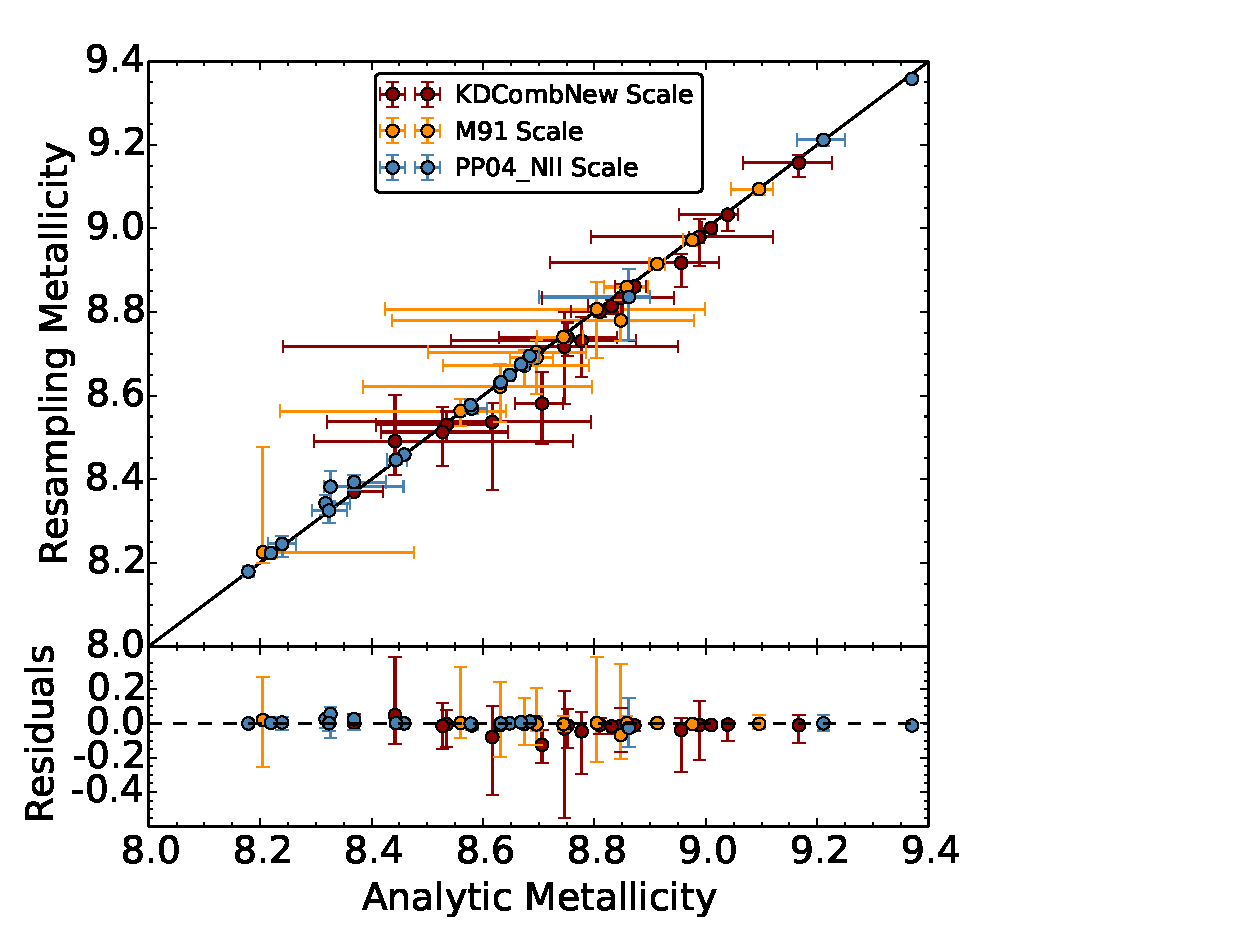
\includegraphics[trim = 10mm 0mm 10mm 0mm, clip]{abcomparison6.eps}
  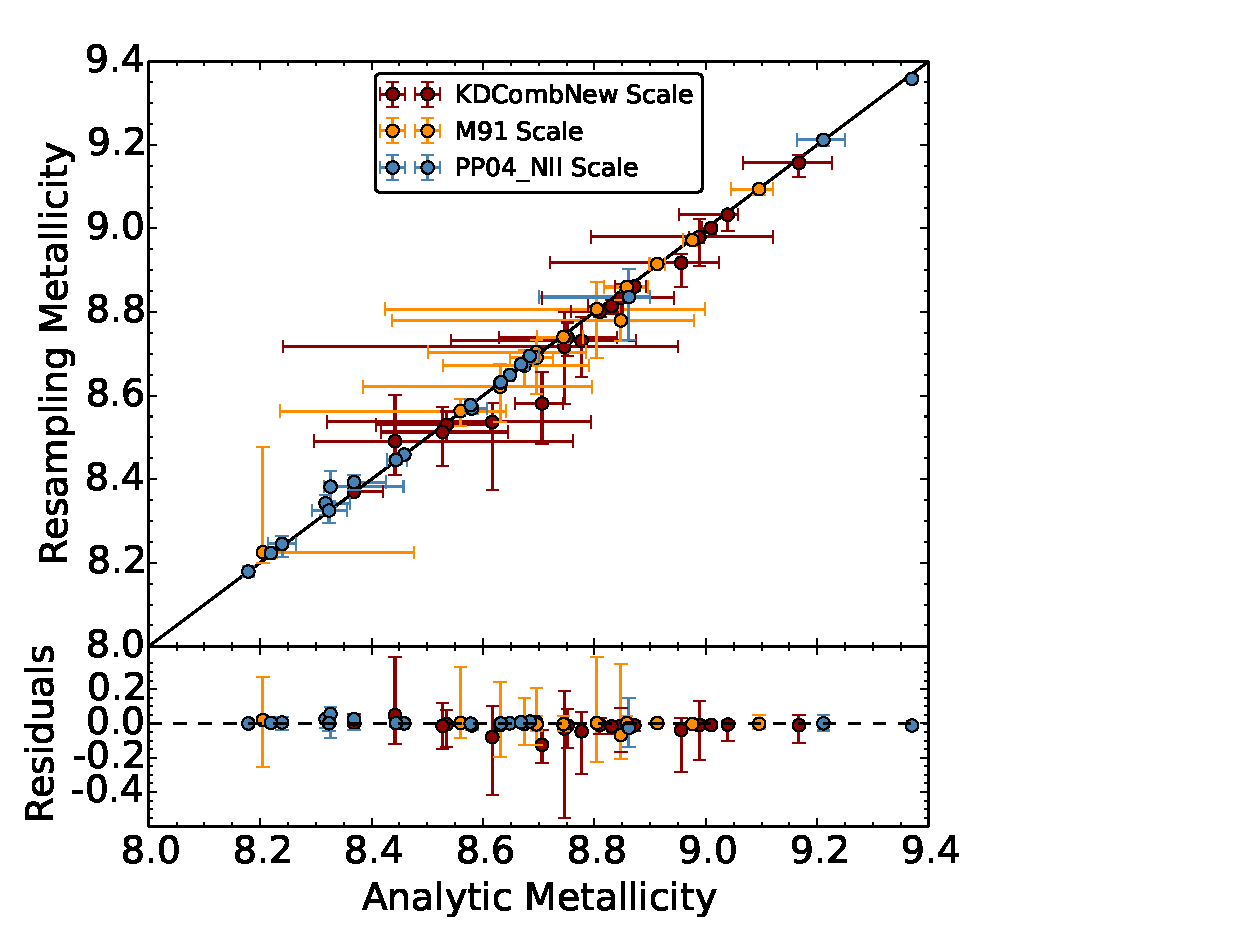
\includegraphics[width=1.2\columnwidth]{abcomparison6.eps}
   \caption{\textbf{FINISH}.Comparison of metallicity estimation between the analytic method and our Monte Carlo resampling method (top) and their residuals (bottom) for 3 different metallicity scales. Flux measurements come from 19 galaxies previously measured in \citet{modjaz11}. To add asymmetric errors in quadrature we use $residual_{min}=\sqrt {x_{max}^2 + y_{min}^2}$ and $residual_{max}=\sqrt {x_{min}^2 + y_{max}^2}$}
 \label{comp_anal_MC}
\end{figure}




%Although the flux probability distribution function is assumed to be symmetric, the metallicity errors are asymmetric because they are derived from the log of minimized and maximized flux ratios.
%Rupke: Errors were propagated primarily using analytic expressions, but for abundance and gradient errors we employed Monte Carlo methods.

\subsection{Comparison with other works}

%Here we perform a literature review of both 


The field of SN host metallicity studies has been rapidly developing as these kinds of studies may be crucial avenues for constraining the progenitor systems of different kinds of explosions - however, a few of the works do not even compute errors and others not show how they compute their statistical errors or  (e.g., \citet{anderson10,leloudas11,sanders12,leloudas14}). While \citet{sanders12} compute the line flux errors from a Markov-Chain Monte Carlo fitting of a gaussian to the emission lines, they only mention in passing that they propagate the line flux uncertainties into the metallicity measurements, but do not describe how {\bf this is a little harsh, right? i think mentioning it without explaining is generally the standard for iid errors -> Maryam: " How would you rephrase it then? " }.

%by propagation of the uncertainties in the line flux measurements
%and the 0.07 dex diagnostic systematic error.
%( line flux errors from MCMC fitting of a gaussian to emission lines)

In contrast, the general metallicity field has considered in detail how to estimate the uncertainties in measured metallicities- however, none of those codes are open-source and many of them are for specific scales which were chosen by the authors:  \citet{moustakas10} also use MC resampling to estimate the metallicity uncertainties (in their case using 500 trials which seems to lead to a Gaussian distribution) but only do this for two scale, KK04 and \citet{pilyugin05}. For computing the metallicities of the SDSS star forming galaxies, \citet{tremonti04} fit a combination of stellar population synthesis and CLOUDY ({\bf citation}) photoionization models to the observed strong emission lines [OII], $H\beta$, [OIII], $H\alpha$, NII and SII and report the median of the metallicity likelihood distribution as the metallicity estimate, with the width of the distribution giving the 1 $\sigma$ (Gaussian) error. However, this is constitutes their own scale (the T04 scale).

In the last stages of preparing this manuscript \citet{blanc15} was published.  \citet{blanc15} employ Bayesian inference for doing something similar to \citet{tremonti04} - they use Bayesian inference to derive the joint and marginalized posterior probability density functions for metallicity $Z$ and ionization parameter $q$ given a set of observed line fluxes and an input photoionization model. They provide a publicly available IDL implementation of their method named $IZI$ (inferring metallicities (Z) and ionization parameters) on the author's website.


\section{Conclusions}\label{comp_sec}

 \textbf{FINISH}. We hope that this open-access code will be used in many different fields where gas-phase metallicities are important, including in the emerging field of SN and GRB host galaxies, where either it is not described how they got  or no error bars are computed (e.g., \citealt{lunnan14}). GIven its public-access nature, the users are free to include any new metallicity diagnostics, e.g., that suggested by \citet{dopita13}.

\acknowledgements
M. Modjaz is supported in parts by the NSF CAREER award AST-1352405 and by NSF award AST-1413260. FBB is supported by a \emph{James Arthur Fellowship} at the NYU-Center for Cosmology and Particle Physics. Some plots are  produced with public code DOI:10.5281/zenodo.15419 available at \url{https://github.com/fedhere/residuals_pylab}.
 This research made use of NASA Astrophysics Data
System; the NASA/IPAC Extragalactic Database (NED), which
is operated by the Jet Propulsion Laboratory, California Institute
of Technology, under contract with the National Aeronautics
and Space Administration.



%\epsscale{1.0}
%\begin{center}
%\csvautotabular{table1.csv}
%\label{t1}
%\caption{Comparison of M-M method with MC method}
%\end{center}
%\end{figure*}



%%%%%%%%%%%%%%%%%%%%%%%%%%%%%%%%%%%%%%%%%%%
%%\clearpage
%%%%%%%%%%%%%%%% BIBLIOGRAPHY  %%%%%%%%%%%%%%%%%%%%%%%% 
\bibliographystyle{apj}
%\bibliography{refs}
\bibliography{refs}

\appendix

\section{Minimum Code validation}
\textbf{WORK WITH FED - and any other code specific things}
\end{document}


@INPROCEEDINGS{astroML,
  author={{Vanderplas}, J.T. and {Connolly}, A.J.
          and {Ivezi{\'c}}, {\v Z}. and {Gray}, A.},
  booktitle={Conference on Intelligent Data Understanding (CIDU)},
  title={Introduction to astroML: Machine learning for astrophysics},
  month={oct.},
  pages={47 -54},
  doi={10.1109/CIDU.2012.6382200},
  year={2012}
}}

@BOOK{astroMLText,
  title={Statistics, Data Mining and Machine Learning in Astronomy},
  author={{Ivezi{\'c}}, {\v Z}. and {Connolly}, A.J.
          and {Vanderplas}, J.T. and {Gray}, A.},
  publisher={Princeton University Press},
  location={Princeton, NJ},
  year={2014}
}

%,page]{appendix}
%\usepackage{amsmath}
%\usepackage{amssymb}
%\usepackage{verbatim}
%\usepackage{graphicx}
%\usepackage{epsfig}
%\usepackage{morefloats}
%\usepackage{float}
%\usepackage{lipsum}
%\usepackage{subfigure}
%\usepackage{longtable}
%\usepackage{lipsum} 
%\usepackage{rotating}
%\usepackage{wasysym}

\begin{document}
\title{Monte Carlo Method for Calculating Uncertainty in Oxygen Abundance from Strong-Line Flux Measurements}

\author{Seung Man Oh\altaffilmark{1,2}, Maryam Modjaz\altaffilmark{1}, David Fierroz\altaffilmark{1}, Federica Bianco\altaffilmark{1}, Yuqian Liu\altaffilmark{1}, Lisa Kewley\altaffilmark{3,4}}
\altaffiltext{1}{Center for Cosmology and Particle Physics, New York University, 4 Washington Place, New York, NY 10003, USA}
 \altaffiltext{2}{NYU Abu Dhabi PO Box 129188 Abu Dhabi, UAE}
 \altaffiltext{3}{Australian National University, Research School for Astronomy \& Astrophysics, Mount Stromlo Observatory, Cotter Road, Weston, ACT 2611, Australia }
 \altaffiltext{4}{ Institute of Astronomy, University of Hawaii, 2680 Woodlawn Drive, Honolulu, HI 96822, USA}
 
 
\begin{abstract}
We present here a Python implementation for the determination of the strong-emission-line estimators of oxygen abundance by \citet{kewley02}. The standard strong line Metallicity scales and diagnostics \text{IMPROVE} have been used to estimate metal abundance by using emission line ratios. Here we introduce Monte Carlo resampling to these methods in order to better characterize an oxygen abundance confidence region.  We output probability distributions, measured values for metallicity and, when desired for reddening E(B-V). We test our code on emission lines measurements from a sample of galaxies ($z<0.15$) and compare our metallicity results with those from previous methods. \textbf{MODIFY AT THE END,}. We show that our metallicity estimate is consistent with previous methods but yields smaller uncertainties. The code is open source and can be found at www.github.com/snyugroup.
\end{abstract}
 
\section{Introduction}
The low quantity of carbon, oxygen, nitrogen, sulfur and iron among other elements provide a splash of color to the otherwise dominating greyscape of hydrogen and helium in the stars and gas of galaxies. Nevertheless, even the minute presence of heavy elements (all elements heavier than H and He, also called metals or collectively metallicity) is important for many areas of astrophysics. For example, \citet{johnson12} suggest that if it was not for the relatively high metallicity level in our solar system, planet formation may not have been possible. With $Z$ representing the mass fraction of metals, for own sun the value is measured to be  Z=0.0153 \citep{chaffau11}, though there are others who suggest a lower solar metallicity of Z=0.0134 in particular because of oxygen \citep{asplund09_rev,grevesse10}\footnote{Note that these abundances refer to the current abundances in the sun, which are lower than the value with which the sun was formed 4.56 Gyr ago, since diffusion at the bottom of the convection zone has decreased metallicity over time \citep{grevesse10}.}. Furthermore, when properly observed and estimated, metallicity measurements of the galactic gas can tightly constrain models of galaxy formation and evolution (e.g., \citealt{kewley08} and references therein), as well as shed light on the metallicity dependence and production conditions for different types of SNe and long-duration GRBs (e.g., \citealt{modjaz08_Z,levesque10_grbhosts,anderson10,modjaz11,kelly12,sanders12}).

%chaffau Z=0.0209 12+log=O/H) = 8.76�0.07 i
%Small variations in chemical abundance can often be critical indicators for stellar and galactic properties like age and activity.
%Metals are produced in the cores of stars during their fusion lifecycle but also during the extreme conditions of stellar explosions. For example, the majority of iron comes from thermonuclear explosions (SN Ia) while nearly all of oxygen is the result of core collapse (SN Ib, Ic, \& II). Since new stars are born from the clouds these explosions produce, metallicity will increase with each passing generation. Stars like our Sun, which are results of multiple generations of star formation, are often found in the more active parts of the galaxy, such as the disk, and are referred to as Population I stars. Population I stars have higher metallicity than older Population II stars, which are also present in the disk but are the exclusive members of the low activity galactic halo. Population III stars would be first generation stars with zero metallicity, but have yet to be observed.
%Besides age, metallicity also influences stellar temperature. Metals are more effective at absorbing energy coming from the interior of the star in the stellar atmosphere so their presence increases the stellar opacity. With greater absorption and opacity the radius expands to a size larger than it would be without metals and this larger size results in a cooler effective temperature. While metallicity can help indicate age or activity it's temperature and density dependencies require parameterization to properly be estimated.

However, for almost all astronomical objects, metallicity cannot be measured directly. The oxygen abundance in the gas-phase is the canonical choice of metallicity indicator for interstellar medium (ISM) studies, since oxygen is the most abundant metal and only weakly depleted onto dust grains (in contrast to refractory elements such as Mg, Si, Fe, with Fe being depleted by more than a factor of 10 in Orion; see \citealt{simondiaz11-orion}). The oxygen abundance\footnote{We note that in many cases in the literature, including here, the terms metallicity and oxygen abundance are used interchangeably.} is expressed as  $12 + \log_{10}(\frac{O}{H})$ where $O$ and $H$ are the number fractions of Oxygen and Hydrogen, respectively. Importantly, oxygen exhibits very strong nebular lines in the optical wavelength range of HII regions (e.g., \citealt{pagel79,osterbrock89,tremonti04}), and thus, well-established diagnostic techniques have been developed (e.g., \citealt{kewley02,pettini04,kobulnicky04,kewley08}). 

\subsection{Oxygen Abundance diagnostics}
The "classical" way to estimate the oxygen abundance is the electron temperature ($T_e$) method, which estimates the electron temperature and density of the nebula using a number of oxygen lines with different ionization states, including the auroral [OIII] $\lambda$4363 line, to then directly estimate the OII and OIII abundances to obtain the total oxygen abundance, after correcting for the unseen stages of ionization. However, the auroral [OIII] $\lambda$4363 line is very weak, even in low-metallicity environments, and saturates at higher metallicity $-$ thus, other methods had to be developed that use other, stronger lines, in the spectra of HII regions. These are called strong-line methods and are the subject of this manuscript. Strong-line methods can be basically categorized into two types: theoretical methods, that rely on calibrating various observed line ratios using photoionization methods (basically theoretically simulating HII regions, using stellar model atmospheres, stellar populations and photoionization models) and empirical ones that calibrate various observed line ratios using observed $T_e$-based metallicities. 


For the theoretical strong-line method, one ratio that is commonly used to determine the metallicity of galaxies is ([OII] $\lambda 3727$ $+$ [OIII] $\lambda 4959,\lambda 5007$)$/$H$_\beta$ \citep{pagel79} and is referred to as R23. The drawback of this method is that it is double-valued with metallicity, and thus other line ratios need to be used to break the degeneracy between the high values ("upper branch") and the low values ("lower branch") of the R23 metallicities. Furthermore, \citet{kewley02} showed the importance of ionization parameter, which can be physically understood to correspond to the maximum velocity of an ionized front that can be driven by the local radiation field of hot massive stars that are ionizing the ISM gas, that needs to be taken into account in the various strong-line methods, as HII regions for the same metallicity but with different ionization parameters produce different line strengths . Calibrations of R23 by \citet{mcgaugh91} (hereafter M91) and by \citet{kewley02} (hereafter KD02) use different theoretical photoionization models and take ionization parameter into account, while other calibrations such as of \citet{zaritsky94} (hereafter Z94) do not. Thus, Z94 is mostly valid for only metal-rich galaxies.  KD02 use an iterative process and two different ratios [NII]$/$[OII] and [NII]$/$H$_\alpha$ to break the R23 degeneracy in order to arrive at the metallicity estimate. 

%The most direct way to estimate metallicity in spectra is to measure line fluxes absorbed or emitted by metals and non-metals. While iron lines may be present in stellar spectra, iron is less commonly found in gaseous nebulae than oxygen is. Not only is oxygen more abundant but it emits several strong lines ([OI] $\lambda 6300$, [OII] $\lambda 3727,7318,7324$, [OIII] $\lambda 4363, 4959, 5007$) visible at optical wavelengths that can also be used to quantify temperature and density. For this reason 
%While the ratio of oxygen to hydrogen line flux correlate with metallicity, the ratio of two [OIII] lines, one auroral $\lambda 4363$ and the other an excitation line at $\lambda 5007$ can be used to determine what is called the Ionization Correction Factor (ICF) (Kewley \& Dopita 2002).
As to empirical strong-line methods, the most commonly used one is by \citet{pettini04} (hereafter PP04). PP04 used HII regions with Te-based metallicities to derive empirical fits to strong-line ratios, and introduce the line ratios of ([NII]$/$H$_\alpha$ (N2) and ([OIII]$/$H$_\beta$)$/$([NII]$/$H$_\alpha$ (O2N2) as metallicity diagnostics. Since PP04-N2 employs two closely spaced lines (Halpha and NII), which are not affected by stellar absorption, nor uncertain reddening, and are easily observed in one simple spectroscopic setup, it has become an often-used scale for at least low-z SN host galaxy studies (e.g. see metal-analysis by e.g,. \citet{sanders12,modjaz12_proc,leloudas14}. However, it is important to remember that this scale has a number of short-comings: it does not take into account the impact of ionization parameter, was initially derived based on only 137 extragalactic HII regions, and the nitrogen emission line employed saturates at high metallicity (CHECK!), and thus this method may not be well-suited for high-metallicity galaxies. An updated calibration by \citet{marino13} based on many more Te-based metallicities (almost three time larger that that of PP04) derives a significantly shallower slope between O3N2 index and oxygen abundance than the PP04 calibration.


As can be seen, each scale has different advantages and disadvantages and may be used in different metallicity regimes (see detailed discussion in e.g.,  \citealt{kewley02,stasinska02,kewley08,moustakas10,dopita13,blanc15}). Thus, this open-source code outputs the oxygen abundance in the main 6 metallicity scales (for which the KD02 diagnostic has four outputs and the PP04 diagnostic has two outputs). While there is a long-standing debate about which diagnostic to use, as there are systematic metallicity offsets between different methods (recombination lines vs.  strong-line method vs. "direct" $T_e$ method, see the above sources), \textbf{the relative metallicity trends can be considered robust, if the analysis is performed self-consistently in the same scale, and trends are seen across different scales \citep{kewley08,moustakas10}}. Note however, that while there are conversion values between different scales \citep{kewley08}, they apply for large data sets, since those conversion values were derived based on ten thousands of SDSS galaxies, and thus should be used with caution (or not at all) for smaller samples. In addition, there the debate about the value of the solar oxygen abundance value \citep{asplund09_rev,chaffau11}, such that the absolute oxygen calibration is still uncertain.



We assume that the observed emission lines to be used to indicate metallicity are from HII regions and are not due to non-thermal excitation by e.g., AGN or interstellar shocks from SNe or stellar winds.  Tests to exclude data contaminated by such non-thermal sources have to be executed by using the recommended line ratios by e.g., \citealt{baldwin81,kauffmann03,kewley06_sdss}. 


Here we introduce the open-source code "". pro .. In \S~\ref{method_sec} we describe our method, the input and output values of the code. In \S~\ref{comp_sec}, we compare our method of obtaining abundance uncertainties to previous methods in the literature. 
%\begin{figure}[H]
%\epsscale{1.0} 
%\begin{center}
%\includegraphics[width=0.89\columnwidth]{fig1.png} 
%\caption{Example of a sampled Gaussian. 50,000 points from a Gaussian distribution were selected in this case}
%\label{f1}
%\end{center}
%\end{figure}


\section{Method}\label{method_sec}

For computing oxygen abundances, we use the iterative code by Kewley \& Dopita (2002), which has been updated in \citet{kewley08} and reflects .. \textbf{LISA: YOUR INPUT HERE:what is the update??} which was initially written in IDL.  We translated it into python, added the new feature of obtaining uncertainties on the metallicity outputs via bootstrap resampling, and made it open source via github, as we explain below.

Emission line flux values are fed into our Python implementation as in the original code by Kewley \& Dopita, which is written in IDL and hereafter referred to as IDL02. The inputs are emission line flux values and their uncertainties for the following lines: H$\alpha$, H$\beta$, [OI] 6300, [OII] 3727, [OIII] 4959, [OIII] 5007, [NII] 6584, [SII] 6717, [SII] 6731, SIII 9532, and SIII 9096 and their uncertainties. If the fluxes for the specified lines are not available, the entry is left to 0 and the outputted oxygen abundance scales will be in only metallicity scales that use the line fluxes provided. 
The inputted line fluxes are corrected for reddening by using the observed Balmer decrement, for which H$\alpha$ and  H$\beta$ flux values are needed to be provided. We assume case B recombination and thus, the standard value of 2.86 as the
intrinsic H$\alpha$/H$\beta$ ratio \citep{osterbrock89}, and apply the standard Galactic reddening law with $R_V$ = 3.1 \citep{cardelli89}. However, the user can choose other extinction laws and $R_V$ values, if desired, given the code's open-source nature.

While other parameters, such as the ionization parameter $q$ and the electron density (using the $SiII$ lines) are computed as long as the necessary lines are provided, they are not outputted in the current version of our code $-$ however, the reader is welcome to easily modify the code to suite their needs, given it's an open-source code.

As output, we obtain metallicity values and their uncertainties in the following calibrations, as discussed in detail in \citet{kewley02,kewley08}: \citet{kewley02}(KD02, for the 4 following computations: R23, using the NIIOII ratio, using the NII/Halpha ratio, and a combined method that uses the optimal method given the input line fluxes), \citet{mcgaugh91} (M91), \citet{zaritsky94} (Z94), \citet{pilyugin01} (P01), \citet{denicolo02} (D02), 
\citet{pettini04} (2 computations: PP04-N2, PP04-O3N2). If the line fluxes necessary for specific scales are not provided, the output will be $-1$.  

The novel aspect of our work is that we introduce a Monte Carlo (MC) algorithm to obtain numerous iterations and random sampling to obtain a more robust result with respect to the uncertainty in the input values. We apply the bootstrapping method which is a resampling technique for error estimation (e.g., \citealt{efron79,hastie09,andrae10}. Given a data set with error bars from which some parameters are estimated, bootstrapping consists of resampling the data to produce alternative data sets. Here we generate a distribution of possible inputs by generating a gaussian distribution centered on the line flux measurement value, with a standard deviation corresponding to the measurement error, where we have made the assumption that the line flux error is gaussian distributed in nature. Every iteration randomly takes an input value from this distribution (for each inputted line) to run the calculations. This effectively emulates conducting multiple experiments when repeated observation is impractical or impossible, as in the case of the emission line flux data, and thus generates alternative data sets. We generated $N$ bootstrap samples of emission line fluxes (where an appropriate value of $N=50,000$ is determined below) and calculated the metallicity for each set of line fluxes. At the end of the iterations, likelihood distributions of the oxygen abundance value are generated for each scale by binning the results to histograms and deriving a confidence region  (see below).

This MC bootstrap approach takes into account the impact of the uncertain reddening (due to the uncertainties in the measurement of the 
H$\alpha$ and H$\beta$ fluxes), when the option for de-reddened metallicities is chosen. Since for each bootstrap iteration, a new reddening value is calculated based on the resampled H$\alpha$ and H$\beta$ fluxes, which is used to compute the de-reddened metallicity value, the derived distribution of metallicity values takes into account the uncertain redding. As part of the optional output, a distribution plot for E(B-V) will be provided, along with confidence intervals  \textbf{add the feature of getting error bars on E(B-V)???}. If either H$\alpha$ or H$\beta$ flux is not provided, then no reddening correction can be applied and the computed metallicity will not be  reddening-corrected. 

However, we note that our code naturally does not include the \emph{systematic} uncertainty of each scale, which are e.g., $\sim$ 0.07 dex for PP04-O2N2.  Thus systematic errors can be as large, if not larger than the statistical errors. 

%However, the
%relative metallicity difference measured between a given pair
%of galaxies in different diagnostics is consistent with an rms
%scatter typically ?0.07 dex, and 0.15 dex between the most
%discrepant diagnostics (Kewley&Ellison 2008).


%from Kewley & Ellison08: The cause of the metallicity calibration discrepancies remains unclear. The discrepancy has been attributed to either an unknown problem with the photoionization models (Kennicutt et al. 2003) or temperature gradients or fluctuations that may cause metallicities based on the electron temperature method to underestimate the true metallicities (Stasin�ska 2002, 2005; Bresolin 2006). Until this discrepancy is resolved, the absolute metallicity scale is uncertain.

\subsection{Histogram Bin Size and Confidence Region}

Choosing the binning for a histogram is not trivial and \citet{hogg08} describes various data analysis recipes for selecting a histogram bin size. Too many bins will result in many empty bins and an "over-fit" histogram, while too few bins may lose features of a probability distribution. Using a bin size of $\sqrt{N}$ was recommended, but this proved to be slightly over-fitting, and after a number of tests, we found $2* \sqrt[3]{N}$ to be appropriate for most cases.

In determining the confidence region interval, there are broadly three approaches (e.g., \citealt{andrae10}): choosing a symmetric interval, the shortest interval , or  a central interval.  We determined the confidence interval using the ``central" method, because it ensures that the algorithm finds the proper boundaries even in the case of multiple peaks (i.e., multimodal likelihood distributions) and for asymmetric, non-Gaussian, distributions. With the "central" method we determined the  confidence interval by choosing the left and right boundaries so that the region outside the confidence interval each equally contains $16\%$ of the total distribution for one standard deviation confidence interval - in analogy to the one-sigma-interval of the Gaussian distribution. While the histograms at sufficiently high $N$, where $N$ is the total number of iterations, yielded single peaked results, at lower $N$ there were occasional multiple peaks resulting from an non-smooth gaussian being sampled. In selecting the value of $N$, we found that around $N=50,000$ provides reliably smooth histograms. The fiftieth (50\%) percentile, i.e.  the median, is reported as the measured value.


\begin{figure*}[!HT]
\epsscale{0.6}
\begin{center}
\centerline{
\includegraphics[width=0.75\columnwidth]{sn2006ss_n50000_KD02_R23_updated_1.pdf}
\includegraphics[width=0.75\columnwidth]{sn2006ss_n50000_KD02comb_updated_1.pdf}
}
\centerline{
\includegraphics[width=0.75\columnwidth]{sn2006ss_n50000_M91_1.pdf}
\includegraphics[width=0.75\columnwidth]{sn2006ss_n50000_PP04_O3N2_1.pdf}
}
\caption{Examples of confidence region determined by the algorithm, shaded in tan color.}
\end{center}
\end{figure*}



\section{Comparison }\label{comp_sec}
(will edit more)
A previous method for determining the uncertainty in the oxygen abundance (as used in \citealt{modjaz08_Z,kewley10,rupke10,modjaz11} was an analytic approach of propagating the emission-line flux uncertainties: it found the difference in maximum and minimum possible abundances via maximizing and minimizing, respectively, the various line ratios. For comparison we computed the metallicities and their errors in these 2 ways (both analytic and using bootstrap) for 3 representative scales. We plot our results and the residuals in Fig.\ref{comp_anal_bootstrap}. There are a number of important points in Fig  MC method has a smaller uncertainty than the analytic method (mean of xx dex). This could be attributed to it reflecting on a more realistic confidence region. The method used the worst case scenario 
Although the flux probability distribution function is assumed to be symmetric, the metallicity errors are asymmetric because they are derived from the log of minimized and maximized flux ratios.

\begin{figure*}[h!]
  \includegraphics[trim = 20mm 0mm 20mm 0mm, clip]{abcomparison2.pdf}
  \caption{Comparison of metallicity estimation between the analytic method and our bootstrap method. Flux measurements come from 19 galaxies previously measured in \citet{modjaz11}. To add asymmetric errors in quadrature we use $residual_{min}=\sqrt {x_{max}^2 + y_{min}^2}$ and $residual_{max}=\sqrt {x_{min}^2 + y_{max}^2}$.}
 \label{comp_anal_bootstrap}
\end{figure*}


Rupke: Errors were propagated primarily using analytic
expressions, but for abundance and gradient errors we employed
Monte Carlo methods.



Here we discuss comparisons with the literature. 

IZI:

\citet{blanc15} employ Bayesian inference for deriving using photoionization codes 
given a set of observed line fluxes and an input
photoionization model

Using the MC method for finding uncertainty in metallicity has been done by  IZI -> FILL IN 
only for one scale and calibration method

Sanders: 
by propagation of the uncertainties in the line flux measurements
and the 0.07 dex diagnostic systematic error.
( line flux errors from MCMC fitting of a gaussian to emission lines)

\section{Conclusions}\label{comp_sec}

\acknowledgements
M. Modjaz is supported in parts by the NSF CAREER award AST-1352405 and by NSF award AST-1413260. 
 This research made use of NASA�s Astrophysics Data
System; the NASA/IPAC Extragalactic Database (NED), which
is operated by the Jet Propulsion Laboratory, California Institute
of Technology, under contract with the National Aeronautics
and Space Administration.

%\begin{figure*}[!H]
%\epsscale{1.0}
%\begin{center}
%\csvautotabular{table1.csv}
%\label{t1}
%\caption{Comparison of M-M method with MC method}
%\end{center}
%\end{figure*}

%\clearpage

%%%%%%%%%%%%%%%%%%%%%%%%%%%%%%%%%%%%%%%%%%%
%%\clearpage
%%%%%%%%%%%%%%%% BIBLIOGRAPHY  %%%%%%%%%%%%%%%%%%%%%%%% 
\bibliographystyle{apj}
%\bibliography{refs}
\bibliography{/Users/maryammodjaz/Dropbox/refs}

\end{document}